\chapter{Investigating the Effects of Radiation Damage on the I320 Intermediate}\label{ch:multi_xtal}

The observation that \atpdx -I320 formed a bridging structure between two active site lysine residues was unexpected, as a structure of this kind had not been observed before. In addition, compounds and cofactors bound to proteins by Schiff bases can be susceptible to site-specific radiation damage, as has been observed in the cases of phosphoserine aminotransferase and bacteriorhodopsin \cite{Dubnovitsky2005,Borshchevskiy2011,Borshchevskiy2014}. This lead to the hypothesis that the bridging structure may be an artefact caused by site-specific radiation damage. If the I320 intermediate was damaged in a site-specific manner during data collection, this would affect the electron density map and may mean that the bridging structure was representative of a damaged state rather than being biologically relevant.

Given that the I320 intermediate is a chromophore, it would be expected that the spectra of the crystals would change if radiation damage affected the chemical structure of the compound. A prominent example of the use of UV-Vis spectroscopy to identify site-specific radiation damage to the prosthetic group of a protein is the radiation-induced isomerisation of rhodopsin in bacteriorhodopsin \cite{Matsui2002,Borshchevskiy2011}. 

UV-Vis spectra of \atpdx -I320 crystals were collected online at ESRF beamline BM30 to determine whether X-ray irradiation resulted in damage to the I320 intermediate. BM30 was chosen due to its top hat beam profile and large beam size which ensured that the crystals were completely and evenly exposed to X-rays. Crystals were continuously exposed to X-rays without rotation of the goniometer, while UV-Vis spectra were collected from the crystals. 

\begin{minipage}{\linewidth}
	\makebox[\linewidth]{
	\includegraphics[width=8cm, height=8cm, keepaspectratio]{/Users/matt/Dropbox/ThesisPrep/Thesis/fig/Ma150-1/Ma150-1pre_spec20overlay.pdf}}	
	\captionof{figure}[Spectra of \atpdx -I320 \textit{in crystallo} pre and post exposure to X-rays]{Spectra of \atpdx -I320 crystal Ma150-1 before exposure to X-rays (blue), and after a total of 800 seconds of X-ray exposure (red). The absorbed dose was calculated to be 48.0 \si{\kilo\gray} using RADDOSE-3D.\label{fig:Ma150-1_I320_pre_20}}	
\end{minipage}

Figure \ref{fig:Ma150-1_I320_pre_20} shows that exposure of \atpdx -I320 crystals to X-rays results in a change in the UV-Vis spectrum of the crystal, the post-exposure crystal has a greater absorbance at 320 \si{\nano\metre}. However, the background absorbance appears to increase, which makes it difficult to interpret whether there is any real change in the amount or state of the I320 present in the crystal.

To identify the sources of the changes in the spectra a series of control experiments were performed on the constituents of the buffer surrounding and within \atpdx -I320 crystals, and on crystals of the \atpdx ~K98A mutant, which is incapable of forming I320 (Section \ref{Sec:SpecRADDAM}).  
\newpage

\section{Identifying the Source of the Radiation Induced Changes in \atpdx -I320 Spectra}\label{Sec:SpecRADDAM}

It is clear that there are changes in the 200 nm - 450 nm region of spectra of \atpdx -I320 crystals when exposed to X-rays (Figure \ref{fig:Ma150-1_I320_pre_20}). The solvents surrounding the crystal were exposed to X-rays, and the changes in the spectra were monitored as a function of X-ray dose to determine whether solvent radiolysis was the source of the changes in the spectra, rather than site specific damage to I320. Any of the constituents of the crystallisation buffer or cryoprotectant solutions may be affected by X-ray radiolysis, leading to the generation of molecules that absorb light in the UV-Vis range and distortion of the crystal spectra. 

\subsection{Irradiation of Water at 100 K}
The major component of the solvent surrounding and within most protein crystals, including those of \atpdx, is water. Comparison of raw spectra collected from ice at different doses shows few changes (Figure \ref{fig:water_norm}). Subtracting the first spectrum collected from each of the spectra collected during the X-ray exposure creates a set of difference spectra; the changes in the spectra of water in response to irradiation are more clearly visible in Figure \ref{fig:water_diff} than Figure \ref{fig:water_norm} with a clear peak forming at 270 nm. Rather than overlaying all of the spectra to understand how the spectra change during X-ray irradiation it is possible to plot all of the difference spectra on a single 3-dimensional heat map (Figure \ref{fig:water_heat}).\\            
\begin{figure}[!htbp]
\centering
\begin{subfigure}{.33\textwidth}
  \centering
  \includegraphics[width=5cm, height=5cm, keepaspectratio]{/Users/matt/Documents/MATLAB/3DPlots/RawSpec/Water_R3_rawplot.pdf}
  \caption{}
  \label{fig:water_norm}
\end{subfigure}%
\begin{subfigure}{.33\textwidth}
  \centering
  \includegraphics[width=5cm, height=5cm, keepaspectratio]{/Users/matt/Documents/MATLAB/3DPlots/DiffSpec/Water_R3_diffplot.pdf}
  \caption{}
  \label{fig:water_diff}
\end{subfigure}
\begin{subfigure}{.33\textwidth}
  \centering
  \includegraphics[width=6cm, height=5cm, keepaspectratio]{/Users/matt/Documents/MATLAB/3DPlots/surf3DwaterADEA.pdf}
  \caption{}
  \label{fig:water_heat}
\end{subfigure}
\caption[UV-Vis Spectra of X-ray Irradiated Water at 100 K]{(a) UV-Vis absorption spectra of a thin film of water at 100 K before X-ray exposure (blue), after absorbing 10 \si{\kilo\gray} (orange) and after absorbing 100 \si{\kilo\gray} (yellow).(b) Spectra of a thin film of water at 100 K immediately before X-ray exposure (blue), after absorbing 10 \si{\kilo\gray} (orange) and after absorbing 100 \si{\kilo\gray} (yellow), with the spectrum of the film collected 100 seconds before the beginning of irradiation subtracted. (c) 3-Dimensional plot showing the change in the UV-Vis spectrum of water at 100 K in response to X-ray irradiation.}
\end{figure}
The most common products of the radiolysis of water are hydrogen radicals, hydroxyl radicals, solvated electrons, hydroxide ions, hydronium ions, hydrogen gas and hydrogen peroxide (Equation \ref{eq:Water_Radiolysis}) \cite{LeCaer2011}. Of the products of water radiolysis, the primary species that absorbs light in the UV-Vis range is the hydroxyl radical (\ce{OH^.}), which has an absorption maximum at 280 \si{\nano\meter} in ice \cite{Ershov1968}. Water molecules, hydrogen peroxide and hydroxyl ions do absorb light in the ultraviolet range, but all have absorption maxima below 200 \si{\nano\meter} and so are not visible in this experiment \cite{Pagsberg1969,Czapski1993}. The difference spectra show a maximum change in absorbance of 0.025 absorbance units at $\sim$ 280 \si{\nano\meter} after a 100 kGy exposure, consistent with the findings of Ershov and Pikaev (Figure \ref{fig:water_heat}) \cite{Ershov1968}. Given the small signal in the difference spectra of water before and after irradiation at 100 K and the dilution of water by buffers and precipitants in the crystallisation buffers it is unlikely that water radiolysis is a major source of the changes observed in \atpdx -I320 crystals. 

%\ce{H2O + hv_{(X-ray)} -> H^{.} ~ OH^{.} ~ e^- ~ OH^- ~ H3O^+ ~ H^2 ~ H2O2}
\begin{equation}
\ce{H2O + hv_{(X-ray)} -> H^{.} + OH^{.} + e^- + OH^ + H3O^+ + H^2 + H2O2}\label{eq:Water_Radiolysis}
\end{equation}

By fitting a Gaussian function to each of the difference spectra in the time series it is possible to monitor how the size of the peak changes with dose and time. Figure \ref{fig:Water_Peak1_Change} shows that the size of the water radiolysis peak increases for the first 400 seconds (52 kGy) of the X-ray exposure before reaching a plateau. After the X-ray shutter is closed at 1800 seconds the size of the peak decreases suggesting that the hydroxyl radicals recombine to form non-chromophoric products. During the X-ray exposure, an equilibrium may be reached with hydroxyl radical formation and recombination occurring at an equal rate.   

\begin{minipage}{\linewidth}
	\makebox[\linewidth]{
	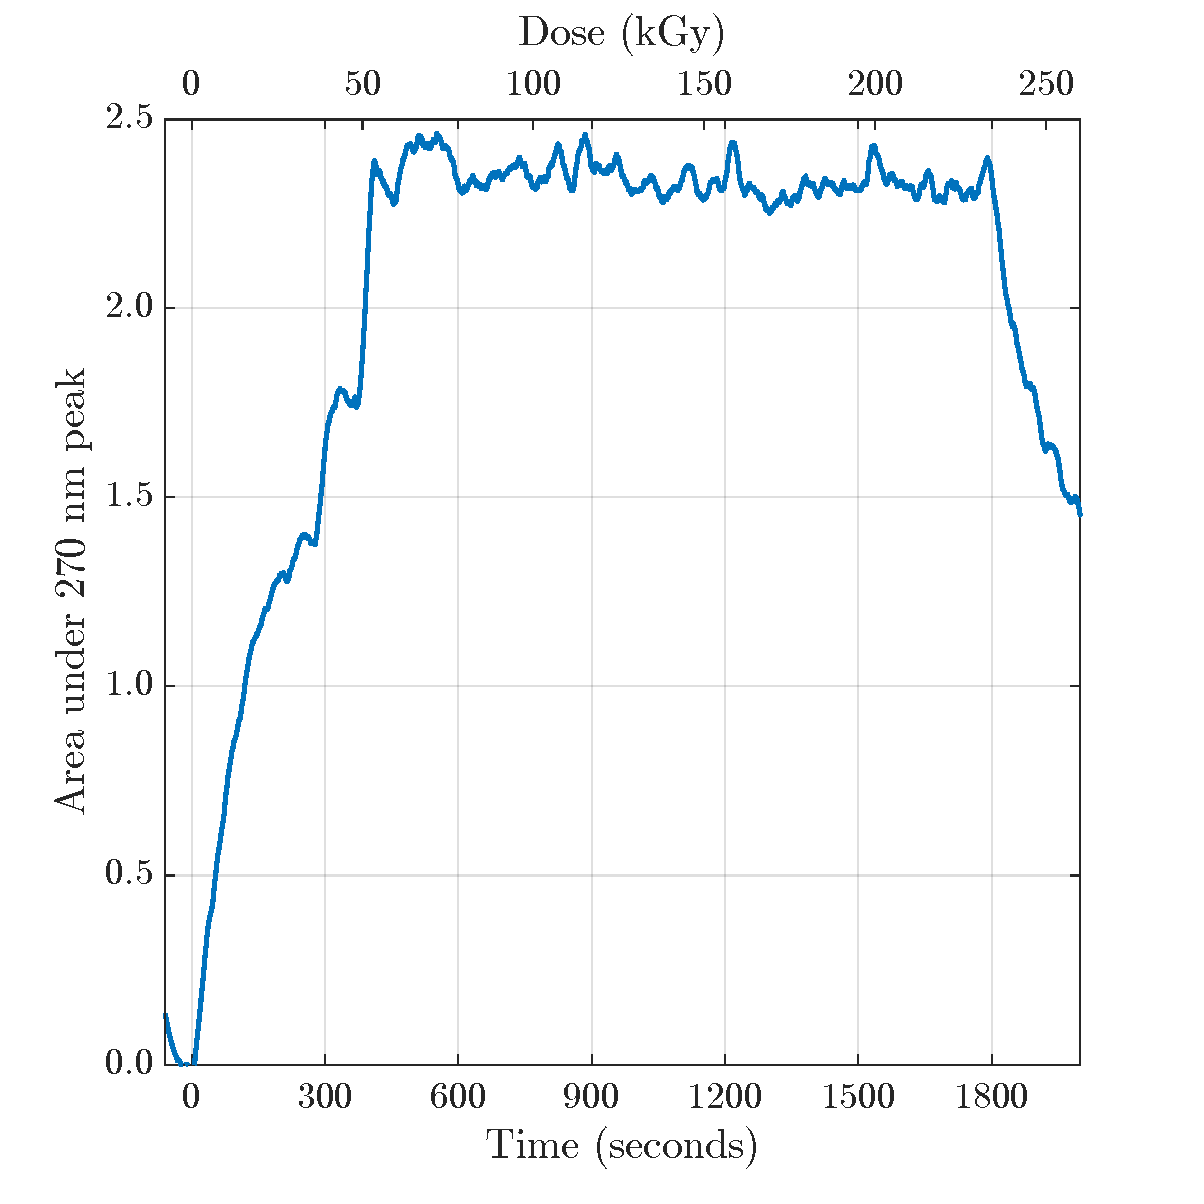
\includegraphics[width=6cm, height=6cm, keepaspectratio]{/Users/matt/Documents/MATLAB/LSQ_Gaussians/Water/PlotgaussianWater.pdf}}	
	\captionof{figure}[]{The peak observed in the water difference spectra had an absorption maximum at 270 nm and a peak sigma of 120 nm. The area under the peak is plotted against time and dose.\label{fig:Water_Peak1_Change}}	
\end{minipage} 
\newpage
\clearpage
\subsection{Irradiation of Glycerol at 100 K}
Glycerol is used as a cryoprotectant in the buffers of the Pdx1 crystals, the role of the cryoprotectant is to prevent the formation of crystalline ice around the crystal during cryocooling. The diffraction of X-rays by multiple randomly oriented ice crystals has a similar effect to that seen in powder diffraction experiments with Debye-Scherrer rings present in the diffraction images; these can obscure diffraction from the protein crystal and complicate data processing. In addition, the formation of ice crystals can disrupt the lattice of the protein crystal and lead to a loss of diffraction. While diffraction is not necessary for these spectroscopy experiments, the presence of ice on the samples also reduces the quality of the spectra obtained, for this reason, the use of a cryoprotectant is necessary.  

Both 100\% and 40\% glycerol were exposed to X-rays to determine the effects of the X-rays on their UV-Vis spectra. Figure \ref{fig:glycerol_series} shows the change in the UV-Vis absorbance spectrum of 100\% glycerol as a response to X-ray irradiation. Two peaks develop as the absorbed dose increases, one with a $\lambda _{max}$= 220 \nm~ and one with a $\lambda _{max}$= 510 \nm ~(Figure \ref{fig:glycerol_diff}). The 40\% glycerol difference spectra also have two peaks, although the peak at 220 nm is relatively small compared to the 100\% glycerol 220 nm peak and the broad peak is shifted to a longer wavelength ($\lambda _{max}$= 590 \nm).\par

\begin{figure}[!htb]
\centering
\begin{subfigure}{.33\textwidth}
  \centering
  \includegraphics[width=5cm, height=5cm, keepaspectratio]{/Users/matt/Documents/MATLAB/3DPlots/RawSpec/Glycerol100_R3_rawplot.pdf}
  \caption{}
  \label{fig:glycerol_series}
\end{subfigure}%
\begin{subfigure}{.33\textwidth}
  \centering
  \includegraphics[width=5cm, height=5cm, keepaspectratio]{/Users/matt/Documents/MATLAB/3DPlots/DiffSpec/GOL100_R3_diffplot.pdf}
  \caption{}
  \label{fig:glycerol_diff}
\end{subfigure}
\begin{subfigure}{.33\textwidth}
  \centering
  \includegraphics[width=6cm, height=5cm, keepaspectratio]{/Users/matt/Documents/MATLAB/3DPlots/surf3DGlycerol100ADEA.pdf}
  \caption{}
  \label{fig:glycerol_3Dplot}
\end{subfigure}
\begin{subfigure}{.33\textwidth}
  \centering
  \includegraphics[width=5cm, height=5cm, keepaspectratio]{/Users/matt/Documents/MATLAB/3DPlots/RawSpec/GOL40_R1_rawplot.pdf}
  \caption{}
  \label{fig:GOL40_norm}
\end{subfigure}%
\begin{subfigure}{.33\textwidth}
  \centering
  \includegraphics[width=5cm, height=5cm, keepaspectratio]{/Users/matt/Documents/MATLAB/3DPlots/DiffSpec/GOL40_R1_R3_diffplot.pdf}
  \caption{}
  \label{fig:GOL40_diff}
\end{subfigure}
\begin{subfigure}{.33\textwidth}
  \centering
  \includegraphics[width=6cm, height=5cm, keepaspectratio]{/Users/matt/Documents/MATLAB/3DPlots/surf3DGlycerol40ADEA.pdf}
  \caption{}
  \label{fig:GOL40_heat}
\end{subfigure}
\caption[UV-Vis Spectra of X-ray Irradiated Glycerol at 100 K]{Spectra were collected from 100\% and 40\% glycerol during irradiation at 100 K and are shown here at doses of 0 kGy (blue), 10 kGy (orange) and 100kGy (yellow). (a) UV-Vis absorption spectra of a thin film of 100\% glycerol. (b) Difference spectra of a thin film of 100\% glycerol. (c) 3-Dimensional plot showing the change in the UV-Vis spectrum of 100\% glycerol at 100 K in response to X-ray irradiation. (d) UV-Vis absorption spectra of a thin film of 40\% glycerol. (e) Difference spectra of a thin film of 40\% glycerol. (f) 3-Dimensional plot showing the change in the UV-Vis spectrum of 40\% glycerol at 100 K in response to X-ray irradiation.}
\end{figure}

The broad peak between 300 nm - 700 nm has previously been observed when glycerol is irradiated with X-rays and is attributed to the absorbance of light by solvated electrons which are generated by the photoelectric effect \cite{McGeehan2009,Owen2011}. Interestingly the absorbance at 530 \nm ~increases for $\sim$ 25 seconds after exposure begins before appearing to decay, despite the X-ray exposure continuing (Figure \ref{fig:glycerol_3Dplot}). The decay of the solvated electron peak has been observed previously, both in investigations into radiolysis of pure glycerol and in cases where protein crystals were cryo-protected in glycerol \cite{Kajiwara1972,Owen2011}. The reaction of the electrons with solvent molecules, causing the formation of anionic radical species, has been identified as the cause of the decline in the solvated electron peak in published pulse radiolysis experiments \cite{LeCaer2016}. The rate of decay and extent to which the absorbance returns to the baseline value was dependent on the composition of the solvent that was irradiated in the previous experiments \cite{LeCaer2016}. %Le Caer \textit{et al} state that recombination of the solvated electrons begins on a picosecond timescale suggesting that the formation of radical species is likely to begin almost instantly \cite{LeCaer2016}. 

It is known from the literature that reducing the glycerol concentration causes the \lwl of the solvated electron peak to shift to longer wavelengths \cite{Ershov1968,McGeehan2009}. McGeehan \textit{et al} showed that the \lwl of the glycerol peak decreased approximately linearly as glycerol concentration increased from $\sim$590 nm in 40\% glycerol to $\sim$490 nm in 100\% glycerol, this finding is supported by similar results in a previous study by Ershov and Pikaev and the results presented here \cite{McGeehan2009,Ershov1968}.        

The absorbance peak at 230 \nm~ increases continuously throughout the period of X-ray irradiation (Figure \ref{fig:glycerol_3Dplot}), previous pulse radiolysis experiments on glycerol showed an increase in absorbance between 245 \nm~ and 270 nm, due to generation of free-radicals by X-ray radiolysis of glycerol \cite{Moore1976}. The \lwl of this peak was dependent on the pH of the glycerol solution and shifted from $\sim$245 nm at pH 5.8 to $\sim$270 nm at pH 11.5 \cite{Moore1976}. 

The product of glycerol radiolysis that has been identified as being primarily responsible for this absorbance change is malondialdehyde \cite{Moore1976,Owen2011,Ivanova2009}. Malondialdehyde is not the final product of glycerol radiolysis as further exposure to X-rays causes it to be oxidised and form $\beta$-oxoacid which has an absorption maximum between 210 \si{\nano\meter} and 230 \si{\nano\meter} \cite{Ivanova2009}. The proposed reaction mechanism for the conversion of glycerol to malondialdehyde is presented in Figure \ref{fig:MDA_mechanism} and is based on Electron Spin Resonance studies of glycerol radiolysis \cite{Ivanova2009,Kuwabara1983,Steenken1974}. 
\FloatBarrier

\begin{figure}[!htbp]
\centering
\begin{subfigure}{.5\textwidth}
  \centering
  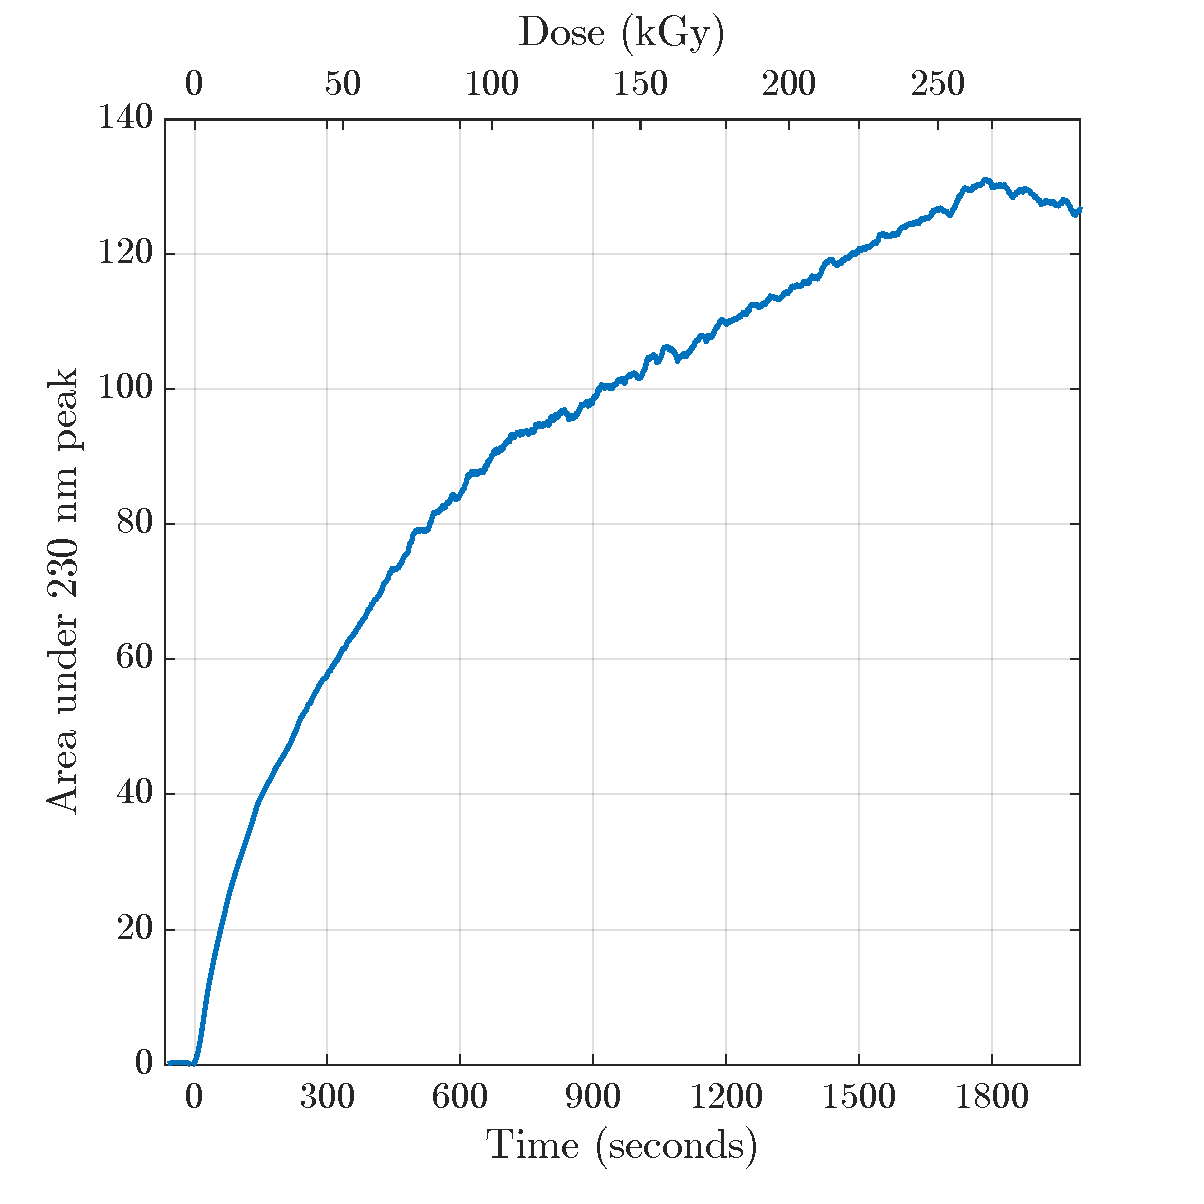
\includegraphics[width=8cm, height=8cm, keepaspectratio]{/Users/matt/Documents/MATLAB/LSQ_Gaussians/glycerol100/PlotGlycerolGaussiansPeak1.pdf}
  \caption{}
  \label{fig:glycerol100_220nm}
\end{subfigure}%
\begin{subfigure}{.5\textwidth}
  \centering
  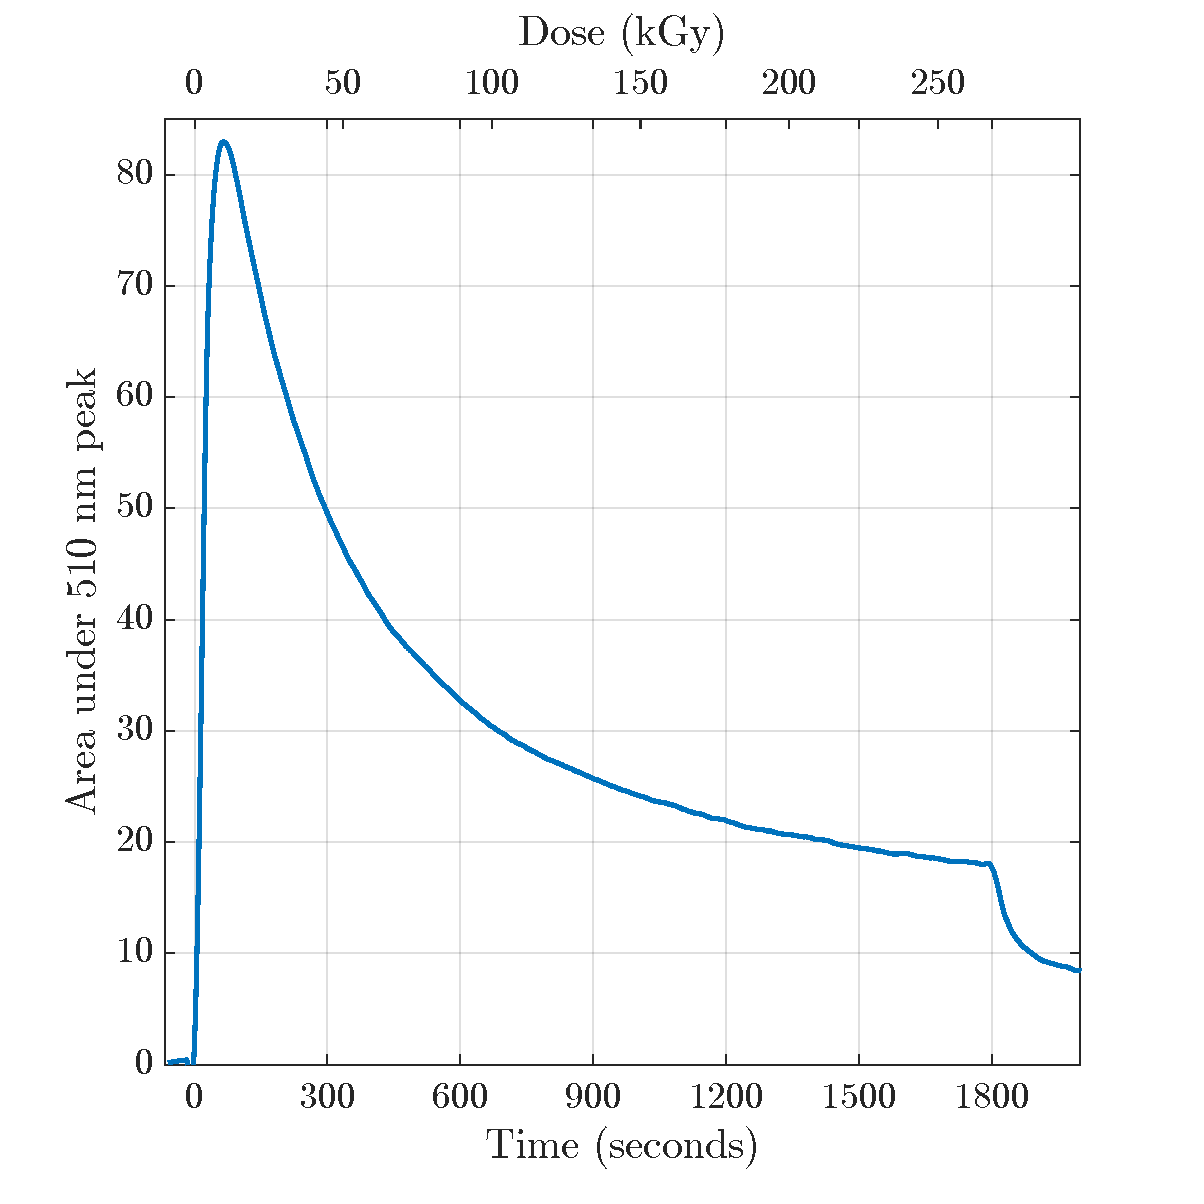
\includegraphics[width=8cm, height=8cm, keepaspectratio]{/Users/matt/Documents/MATLAB/LSQ_Gaussians/glycerol100/PlotGlycerolGaussiansPeak2.pdf}
  \caption{}
  \label{fig:glycerol_530nm}
\end{subfigure}
\begin{subfigure}{.5\textwidth}
  \centering
  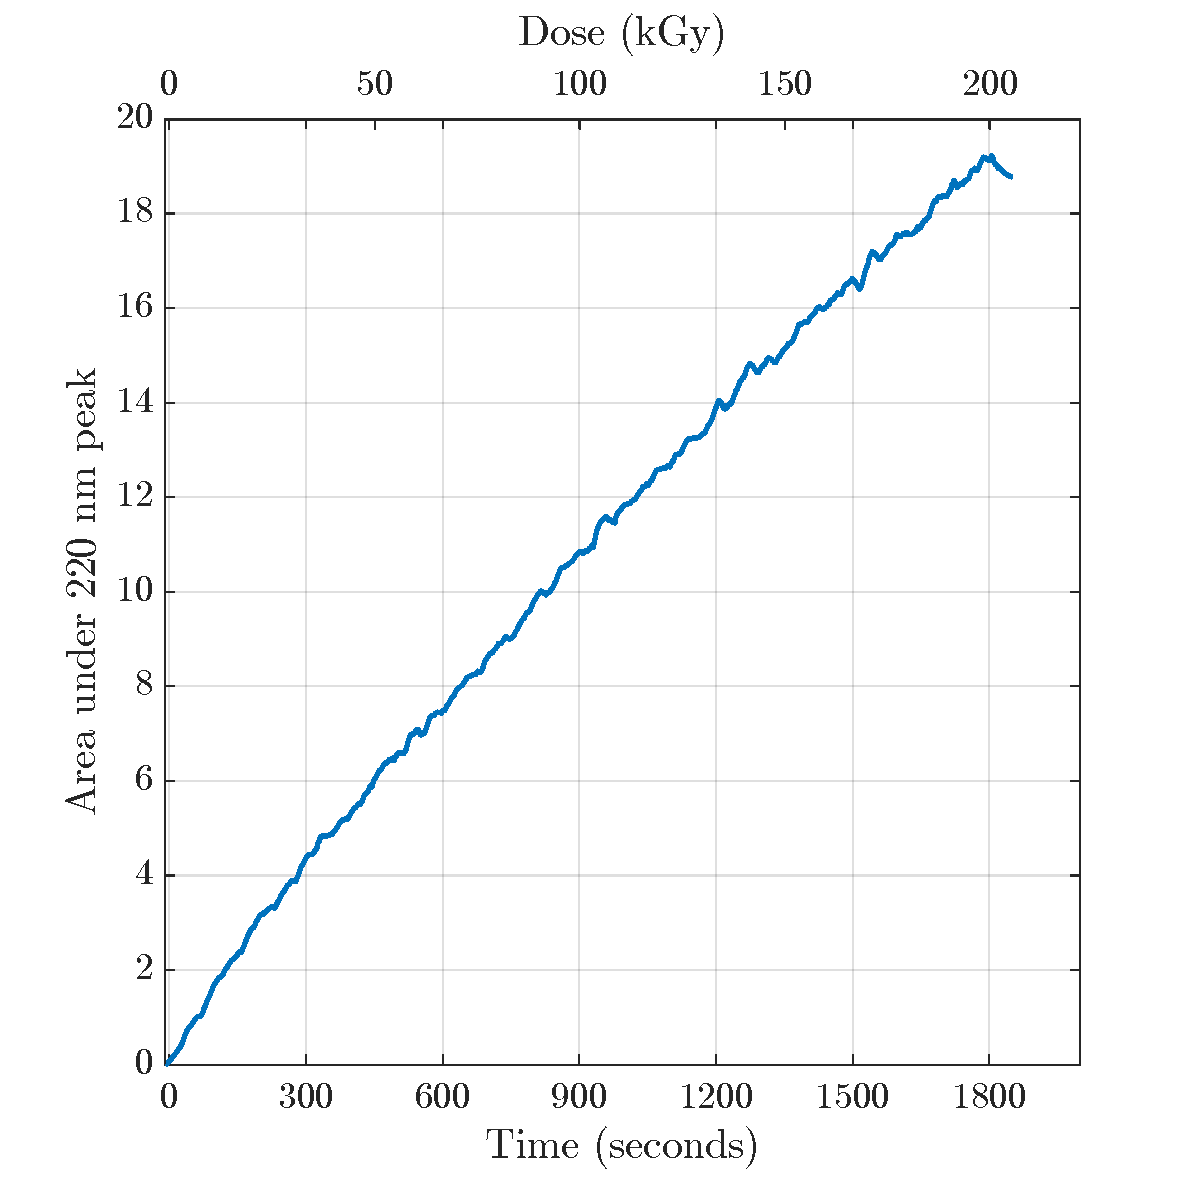
\includegraphics[width=8cm, height=8cm, keepaspectratio]{/Users/matt/Documents/MATLAB/LSQ_Gaussians/Glycerol40/PlotGlycerol40Peak1.pdf}
  \caption{}
  \label{fig:glycerol40_220nm}
\end{subfigure}%
\begin{subfigure}{.5\textwidth}
  \centering
  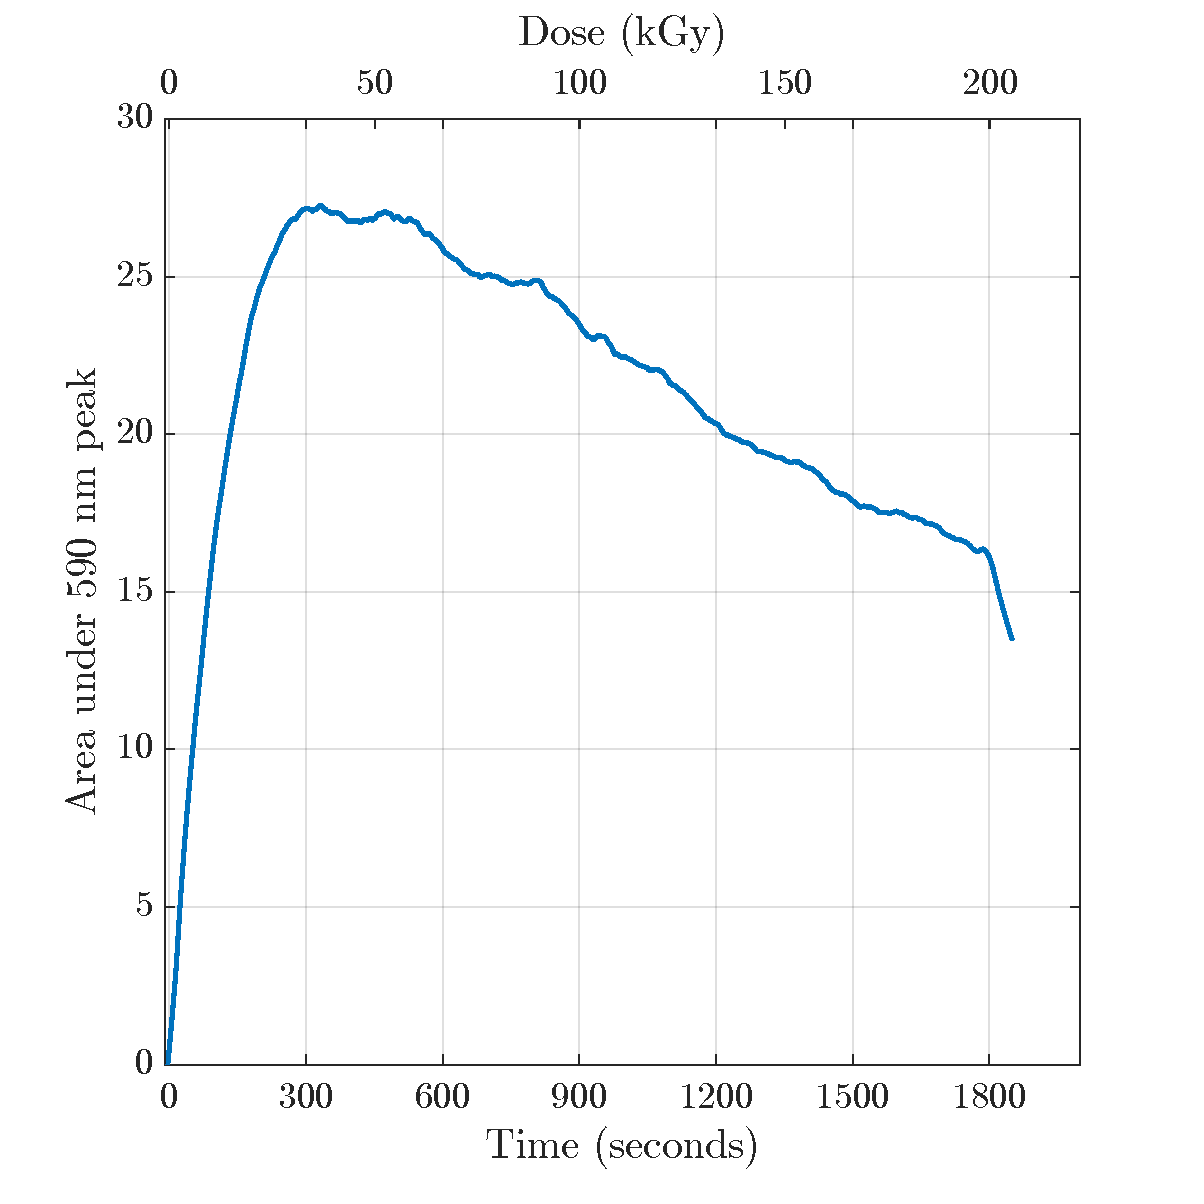
\includegraphics[width=8cm, height=8cm, keepaspectratio]{/Users/matt/Documents/MATLAB/LSQ_Gaussians/Glycerol40/PlotGlycerol40Peak2.pdf}
  \caption{}
  \label{fig:glycerol40_590nm}
\end{subfigure}
\caption[]{The peaks observed in the 100\% glycerol difference spectra had absorption maxima at 230 nm (a) and 530 nm (b). The peaks in the 40\% glycerol difference spectra had absorption maxima at 230 nm (c) and 590 nm (d). The area under each peak is plotted against time and dose.}
\end{figure}
% 
%\par 

\begin{minipage}[!htp]{\linewidth}
	\makebox[\linewidth]{
	\includegraphics[width=12cm, keepaspectratio]{/Users/matt/Dropbox/ThesisPrep/Thesis/fig/reactionsceme/Glycerol2MalonylReactioncrop.pdf}}	
	\captionof{figure}[Reaction Mechanism for Conversion of Glycerol to Malondialedhyde]{The abstraction of a hydrogen atom from glycerol (1) by a hydroxyl radical produces a glycerol radical (2) and a molecule of water \cite{Steenken1974}. A water molecule is spontaneously eliminated from the glycerol radical to form a dehydrated glycerol radical (3), this reaction may be acid catalysed \cite{Steenken1974}. A hydrogen atom is transferred from one dehydrated glycerol radical to another this produces one molecule of 3-hydroxypropanal (4) and one molecule of 3-hydroxyacrylaldehyde (5) \cite{Ivanova2009}. 3-hydroxyacrylaldehyde reversibly tautomerises to malondialdehyde (6) which absorbs light in the UV-Vis range (\lwl 260 nm) \cite{Ivanova2009}. \label{fig:MDA_mechanism}}	
\end{minipage}
\FloatBarrier
\clearpage
\subsection{Irradiation of 2-Methyl-2,4-pentanediol (MPD) at 100 K}

It has previously been identified that MPD, another commonly used cryoprotectant, does not display a strong peak for solvated electrons during X-ray irradiation \cite{McGeehan2009,Owen2011}. If MPD could be substituted for glycerol as a cryoprotectant, this would be a method for collecting spectra of \atpdx -I320 without the effect on the spectra caused by the generation of solvated photoelectrons as observed with glycerol (Figure \ref{fig:glycerol_3Dplot}). This would also be helpful in investigations into the effects of X-rays on proteins with a chromophore such as haem and rhodopsin which have a \lwl between 400 nm and 700 nm and have been identified as being affected by site specific radiation damage through the use of \textit{in crystallo} UV-Vis spectroscopy \cite{Borshchevskiy2011,Hersleth2011}. In the case of site specific radiation damage to haem in myoglobin Hersleth \textit{et al} had difficulty separating the effects of absorption of light by solvated photoelectrons from the effects of radiation damage when glucose and glycerol were used as cryoprotectants. The use of MPD as a cryoprotectant may circumvent this problem \cite{Hersleth2011}.

While the solvated electron peak in irradiated glycerol does not strongly overlap with the I320 peak or complicate interpretation of the spectra, the 220 nm peak does. If the 220 nm peak was absent in difference spectra of irradiated MPD there would be a clear advantage to using MPD as a cryoprotectant in the experiments investigating the effect of irradiation on the UV-Vis spectra of \atpdx -I320 crystals.   

Figure \ref{fig:MPD100_3Dplot} shows that if there is any absorbance of light by solvated electrons between 400 \si{\nano\meter} - 700 \si{\nano\meter} in 100\% MPD, as observed by Owen \textit{et al} with 50\% MPD, it has a negligible effect on the spectra. However, the solvated electron peak is visible in the 40\% MPD data with a \lwl $\sim$600 nm (Figure  \ref{fig:MPD40_3Dplot}). The magnitude of this solvated electron peak is smaller than that observed in glycerol by a factor of $\sim$10.  

A peak at $\sim$220 nm develops over the course of the experiment and may be caused by the formation of a similar compound to the $\beta$-oxoacid that is generated by during glycerol radiation; however, this cannot be confirmed without the use of EPR to analyse the products of MPD irradiation. The determination of the compound responsible for the absorbance peak $\sim$220 nm in irradiated glycerol was considered to be outside the scope of this investigation. Due to the noisiness of the 40\% MPD data, it was not possible to produce a meaningful fit of the data to a Gaussian function; however, it was possible for the 100\% MPD data. Figure \ref{fig:MPD100peak} shows a similar trend to that of the 100\% glycerol data with the rate of increase in the size of the 224 nm peak the greatest at the start of irradiation.

As the peak $\sim$220 nm is present in the difference spectra of both glycerol and MPD, there does not appear to be a clear advantage to using one instead of the other as a cryoprotectant for the spectroscopy experiments investigating the effect of irradiation on \atpdx -I320 crystals.    
  
\begin{figure}[!htbp]
\centering
\begin{subfigure}{.33\textwidth}
  \centering
  \includegraphics[width=5cm, height=5cm, keepaspectratio]{/Users/matt/Documents/MATLAB/3DPlots/RawSpec/MPD40_R3_rawplot.pdf}
  \caption{}
  \label{fig:MPD40_raw}
\end{subfigure}%
\begin{subfigure}{.33\textwidth}
  \centering
  \includegraphics[width=5cm, height=5cm, keepaspectratio]{/Users/matt/Documents/MATLAB/3DPlots/DiffSpec/MPD40_R3_diffplot.pdf}
  \caption{}
  \label{fig:MPD40_diff}
\end{subfigure}
\begin{subfigure}{.33\textwidth}
  \centering
  \includegraphics[width=6cm, height=5cm, keepaspectratio]{/Users/matt/Documents/MATLAB/3DPlots/surf3DMPD40ADEA.pdf}
  \caption{}
  \label{fig:MPD40_3Dplot}
\end{subfigure}
\begin{subfigure}{.33\textwidth}
  \centering
  \includegraphics[width=5cm, height=5cm, keepaspectratio]{/Users/matt/Documents/MATLAB/3DPlots/RawSpec/MPD100_R1_rawplot.pdf}
  \caption{}
  \label{fig:MPD100_raw}
\end{subfigure}%
\begin{subfigure}{.33\textwidth}
  \centering
  \includegraphics[width=5cm, height=5cm, keepaspectratio]{/Users/matt/Documents/MATLAB/3DPlots/DiffSpec/MPD100_R1_diffplot.pdf}
  \caption{}
  \label{fig:MPD100_diff}
\end{subfigure}
\begin{subfigure}{.33\textwidth}
  \centering
  \includegraphics[width=6cm, height=5cm, keepaspectratio]{/Users/matt/Documents/MATLAB/3DPlots/surf3DMPD100ADEA.pdf}
  \caption{}
  \label{fig:MPD100_3Dplot}
\end{subfigure}
\caption[UV-Vis Spectra of X-ray irradiated 40\% and 100\% MPD]{Spectra were collected from 40\%  and 100\% MPD during irradiation at 100 K and are shown here at doses of 0 kGy (blue), 10 kGy (orange) and 100kGy (yellow). (a) UV-Vis absorption spectra of a thin film of 40\% MPD during X-ray irradiation. (b) Difference spectra of a thin film of 40\% MPD at 0 kGy, 10 kGy and 100 kGy. (c) 3-Dimensional plot showing the change in the UV-Vis spectrum of 40\% MPD at 100 K in response to X-ray irradiation. (d) UV-Vis absorption spectra of a thin film of 100\% MPD during X-ray irradiation. (e) Difference spectra of a thin film of 100\% MPD at 0 kGy, 10 kGy and 100 kGy. (f) 3-Dimensional plot showing the change in the UV-Vis spectrum of 100\% MPD at 100 K in response to X-ray irradiation.}
\end{figure}  

\begin{minipage}{\linewidth}
	\makebox[\linewidth]{
	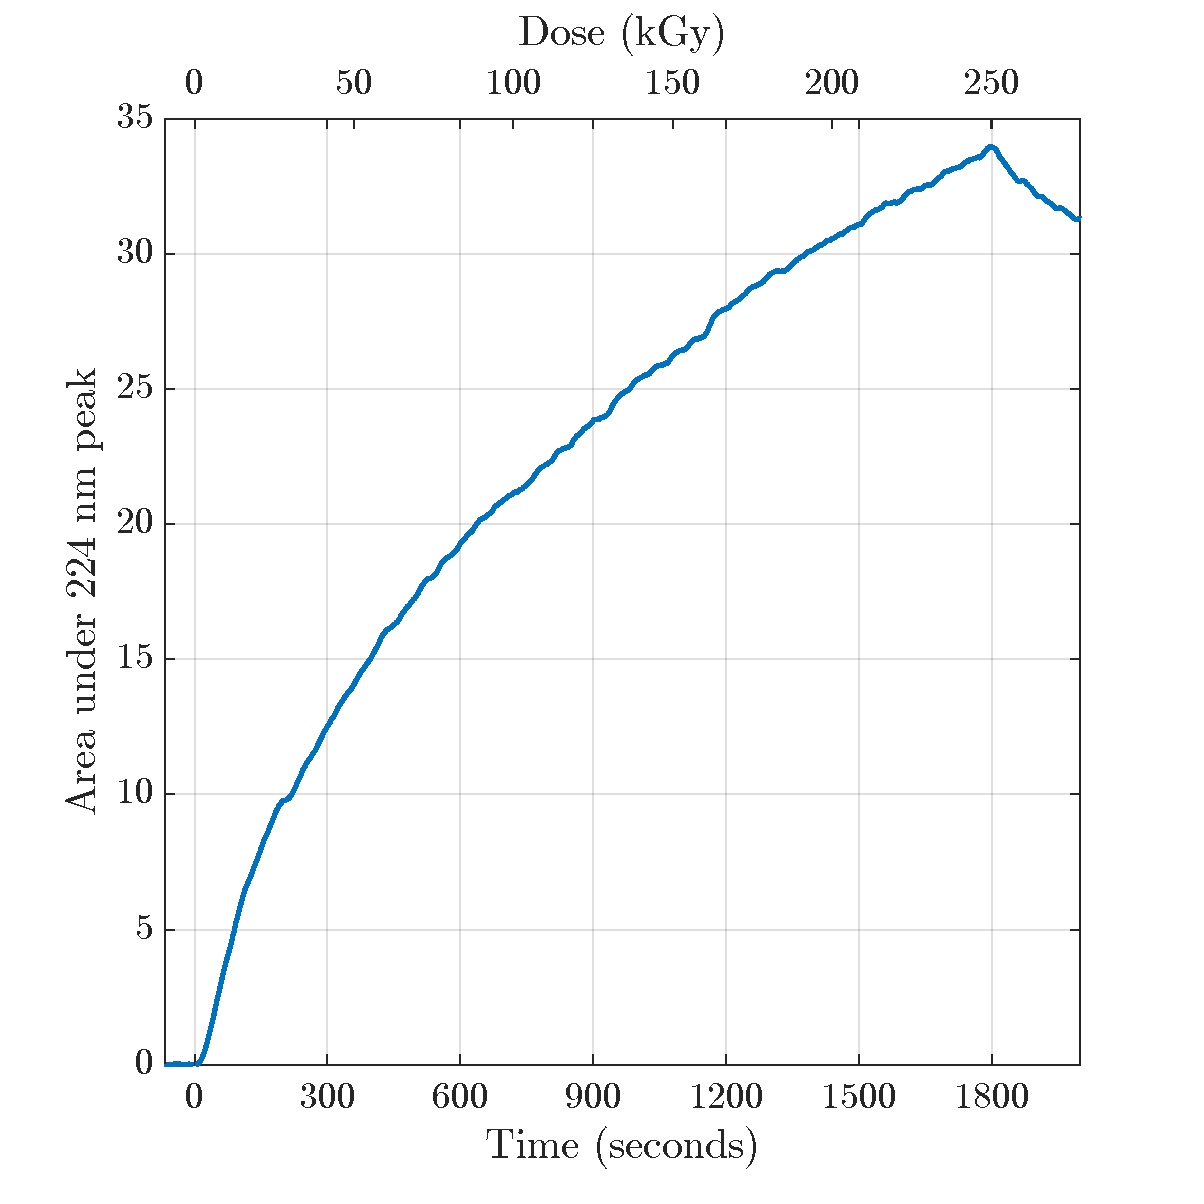
\includegraphics[width=8cm, height=8cm, keepaspectratio]{/Users/matt/Documents/MATLAB/LSQ_Gaussians/MPD100/MPD100Peak1.pdf}}	
	\captionof{figure}[Formation of a 224 nm peak during irradiation of 100\% MPD]{A peak forms with an absorption maximum at 224 nm when 100\% MPD is exposed to X-rays. The area under the peak is plotted against time and dose.\label{fig:MPD100peak}}	
\end{minipage}
  
\FloatBarrier
\clearpage
\subsection{Irradiation of the \atpdx -I320 Cryobuffer at 100 K}
In addition to water and glycerol the cryobuffer that the \atpdx -I320 crystals were mounted in contained PEG 4000, sodium acetate and Tris. Comparison of the cryobuffer spectra with those of 40\% and 100\% glycerol enables identification of peaks that develop as a result of radiolysis of the buffers and precipitants used for crystallisation.   

\begin{figure}[!htbp]
\centering
\begin{subfigure}{.33\textwidth}
  \centering
  \includegraphics[width=5cm, height=5cm, keepaspectratio]{/Users/matt/Documents/MATLAB/3DPlots/RawSpec/A4Buffer_rawplot.pdf}
  \caption{}
  \label{fig:A4Buffer_raw}
\end{subfigure}%
\begin{subfigure}{.33\textwidth}
  \centering
  \includegraphics[width=5cm, height=5cm, keepaspectratio]{/Users/matt/Documents/MATLAB/3DPlots/DiffSpec/A4Buffer_diffplot.pdf}
  \caption{}
  \label{fig:A4Buffer_diff}
\end{subfigure}
\begin{subfigure}{.33\textwidth}
  \centering
  \includegraphics[width=6cm, height=5cm, keepaspectratio]{/Users/matt/Documents/MATLAB/3DPlots/surf3DcryobufferADEA.pdf}
  \caption{}
  \label{fig:A4Buffer_3Dplot}
\end{subfigure}
\begin{subfigure}{.33\textwidth}
  \centering
  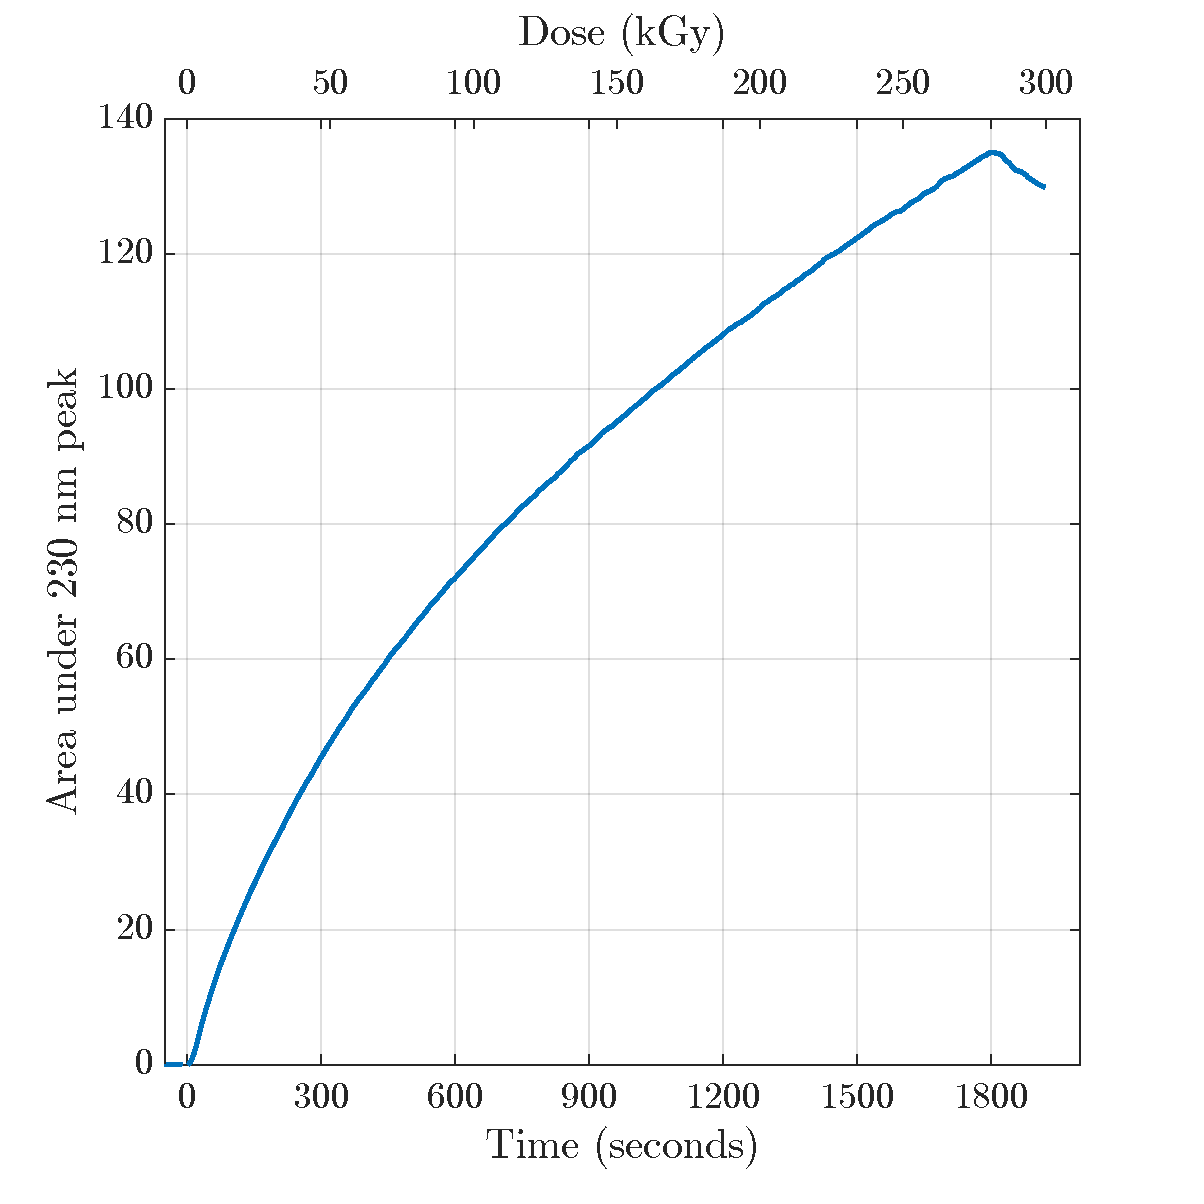
\includegraphics[width=5cm, height=5cm, keepaspectratio]{/Users/matt/Documents/MATLAB/LSQ_Gaussians/A4Cryo/PlotA4CryoGaussiansPeak1.pdf}
  \caption{}
  \label{fig:A4Buffer_Peak1}
\end{subfigure}
\begin{subfigure}{.33\textwidth}
  \centering
  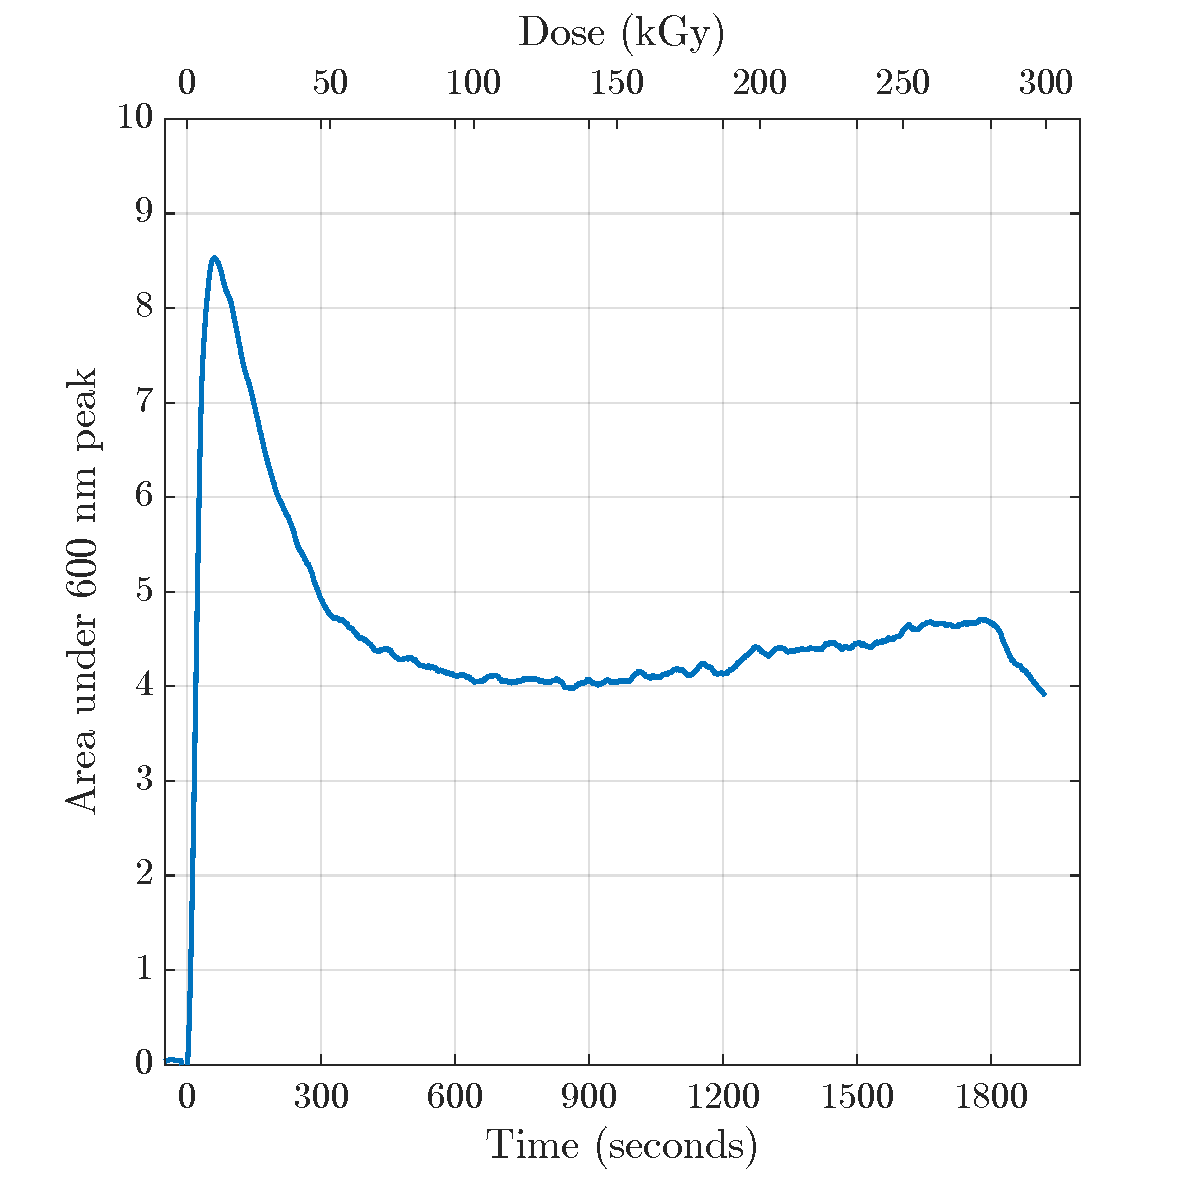
\includegraphics[width=5cm, height=5cm, keepaspectratio]{/Users/matt/Documents/MATLAB/LSQ_Gaussians/A4Cryo/PlotA4CryoGaussiansPeak2.pdf}
  \caption{}
  \label{fig:A4Buffer_Peak2}
\end{subfigure}
\caption[UV-Vis Spectra of X-ray irradiated cryobuffer solution]{(a) UV-Vis absorption spectra of a thin film of the Pdx1 cryobuffer at 100 K before X-ray exposure (blue), after absorbing 10 \si{\kilo\gray} (orange) and after absorbing 100 \si{\kilo\gray} (yellow). (b) Difference spectra of a thin film of cryobuffer solution immediately before X-ray exposure (blue), after absorbing 10 \si{\kilo\gray} (orange) and after absorbing 100 \si{\kilo\gray} (yellow). (c) 3-Dimensional plot showing the change in the UV-Vis spectrum of the cryobuffer solution in response to X-ray irradiation. (d) Change in size of the 230 nm peak during X-ray irradiation. (e) Change in size of 600 nm peak during X-ray irradiation.}
\end{figure}

The spectra of the cryobuffer appear to be similar to that of the glycerol solutions, a peak is visible at 220 nm, as is a second broad peak with a \lwl $\sim$600 nm (Figure \ref{fig:A4Buffer_3Dplot}). The shift in \lwl of the solvated electron peak from 590 nm in 40\% glycerol to 600 nm in the cryobuffer is likely to be caused by the concentration of glycerol in the buffer being 20\% lower. This result suggests that if the PEG 4000, sodium acetate and Tris are being affected by the radiation, the products that they are forming do not absorb light significantly in the UV-Vis range.
\FloatBarrier
\clearpage
\subsection{Irradiation of \atpdx~ K98A crystals at 100 K}
A control experiment was performed using crystals of the K98A mutant, to determine whether the spectroscopic changes observed when \atpdx -I320 crystals were irradiated was caused by changes in the protein structure or damage to I320. The K98A mutant was chosen as it has been shown to be incapable of forming a covalent complex with R5P or catalysing I320 formation (Section \ref{sec:K98A}). Any change in the spectra of these crystals should, therefore, be attributable either to reaction products of solvent radiolysis or damage to the protein itself.  

It is expected that if the difference spectra show the same changes in the spectra as the cryobuffer (Figure \ref{fig:A4Buffer_3Dplot}), then the only source of the changes in the spectra is solvent radiolysis. 
    
\begin{figure}[!htbp]
\centering
\begin{subfigure}{.33\textwidth}
  \centering
  \includegraphics[width=5cm, height=5cm, keepaspectratio]{/Users/matt/Documents/MATLAB/3DPlots/RawSpec/K98Acrystal_rawplot.pdf}
  \caption{}
  \label{fig:K98ACrystal_raw}
\end{subfigure}%
\begin{subfigure}{.33\textwidth}
  \centering
  \includegraphics[width=5cm, height=5cm, keepaspectratio]{/Users/matt/Documents/MATLAB/3DPlots/DiffSpec/K98Acrystal_diffplot.pdf}
  \caption{}
  \label{fig:K98ACrystal_diff}
\end{subfigure}
\begin{subfigure}{.33\textwidth}
  \centering
  \includegraphics[width=6cm, height=5cm, keepaspectratio]{/Users/matt/Documents/MATLAB/3DPlots/surf3DK98AcrystalADEA.pdf}
  \caption{}
  \label{fig:K98ACrystal_3Dplot}
\end{subfigure}
\caption[UV-Vis Spectra of an X-ray irradiated \atpdx~ K98A crystal]{(a) UV-Vis absorption spectra of an \atpdx~ K98A crystal at 100 K before X-ray exposure (blue), after absorbing 10 \si{\kilo\gray} (orange) and after absorbing 100 \si{\kilo\gray} (yellow). (b) Difference spectra of an \atpdx~ K98A crystal immediately before X-ray exposure (blue), after absorbing 10 \si{\kilo\gray} (orange) and after absorbing 100 \si{\kilo\gray} (yellow). (c) 3-Dimensional plot showing the change in the UV-Vis spectrum of the cryobuffer solution in response to X-ray irradiation.}
\end{figure}

The difference spectrum of \atpdx~ K98A at 100 kGy shows three main features, a peak at $\sim$235 nm with a shoulder at $\sim$310 nm, and a broad peak at $\sim$600 nm (Figure \ref{fig:K98ACrystal_diff}). Given that the solvent surrounding \atpdx ~K98A crystals contains 20\% glycerol it is likely that the 235 nm and 600 nm peaks are caused by glycerol radiolysis and generation of solvated electrons.

As we know that the K98A mutant is incapable of forming the I320 intermediate, it is possible to exclude site-specific radiation damage to I320 as a cause for the formation of the 310 nm peak. The peak is absent in the difference spectra for the cryobuffer (Figure \ref{fig:A4Buffer_diff}) and is, therefore, likely to be formed as a result of damage to the protein. On the basis of the results shown here, it is not possible to identify a particular amino acid that is likely to be the source of the change in the spectra.   

\FloatBarrier
\clearpage
\subsection{Irradiation of \atpdx -I320 ~crystals at 100 K}
The raw spectrum of an \atpdx -I320 crystal before irradiation appears as may be expected; a strong peak at 220 nm caused by absorbance by the peptide backbone, a second peak at 280 nm caused by absorption by the aromatic residues and a third peak at 320 nm due to the presence of the I320 intermediate (Figure \ref{fig:I320GOLCrystal_raw}, blue). 

Similarly to the \atpdx ~K98A spectra, the difference spectra of \atpdx -I320 during irradiation also show an intense peak at $\sim$235 nm, due to glycerol radiolysis, a transient solvated electron peak at $\sim$600 nm and a slight shoulder at 310 nm caused by an unknown damage process involving the protein. 

While these results suggest that radiation damage to the I320 intermediate does not occur within the first 250 kGy of irradiation, the results are not entirely conclusive, as any change in absorbance by the I320 intermediate may be obscured by the effects of solvent radiolysis. To gain a greater understanding of whether site specific radiation damage has an effect on the structure of the I320 intermediate, it was decided to solve the structure at a dose below 200 kGy, which is the dose range in which these spectral changes are taking place. Section \ref{sec:MultiXtal} describes the experiments performed to solve the \atpdx -I320 structure at low dose improve our understanding of how the structure of the protein changes in response to the absorption of X-rays. 
  
\begin{figure}[!htbp]
\centering
\begin{subfigure}{.33\textwidth}
  \centering
  \includegraphics[width=5cm, height=5cm, keepaspectratio]{/Users/matt/Documents/MATLAB/3DPlots/RawSpec/Ma275_1crystal_rawplot.pdf}
  \caption{}
  \label{fig:I320GOLCrystal_raw}
\end{subfigure}%
\begin{subfigure}{.33\textwidth}
  \centering
  \includegraphics[width=5cm, height=5cm, keepaspectratio]{/Users/matt/Documents/MATLAB/3DPlots/DiffSpec/Ma275_1crystal_diffplot.pdf}
  \caption{}
  \label{fig:I320GOLCrystal_diff}
\end{subfigure}
\begin{subfigure}{.33\textwidth}
  \centering
  \includegraphics[width=6cm, height=5cm, keepaspectratio]{/Users/matt/Documents/MATLAB/3DPlots/surf3DMa275_2crystalADEA.pdf}
  \caption{}
  \label{fig:I320GOLCrystal_3Dplot}
\end{subfigure}
\caption[UV-Vis Spectra of X-ray irradiated \atpdx -I320 crystals]{(a) UV-Vis absorption spectra of a wild type \atpdx -I320 crystal at 100 K before X-ray exposure (blue), after absorbing 10 \si{\kilo\gray} (orange) and after absorbing 100 \si{\kilo\gray} (yellow).(b) Difference spectra of an \atpdx -I320 crystal immediately before X-ray exposure (blue), after absorbing 10 \si{\kilo\gray} (orange) and after absorbing 100 \si{\kilo\gray} (yellow). (c) 3-Dimensional plot showing the change in the UV-Vis spectrum of the cryobuffer solution in response to X-ray irradiation.}
\end{figure}

\clearpage

\section{Using Multi-Crystal Techniques to Investigate Radiation Damage}
\label{sec:MultiXtal}
The changes in the spectra of the \atpdx -I320 crystals are taking place within the first few hundred kilograys of X-ray exposure (Figure \ref{fig:I320GOLCrystal_3Dplot}). Radiolysis of solvent molecules such as glycerol or water are unlikely to be visible in the electron density maps for \atpdx -I320 as the vast majority of these molecules in the crystal are not present in an ordered position that is consistent across unit cells. In contrast, any specific radiation damage taking place in ordered components of the unit cell, such as the majority of the amino acids in the protein and the ligands such as I320 will be visible as a change in the electron density surrounding the damaged atoms. 

It is necessary to solve the structure in a relatively undamaged state and compare that structure to the damaged state to observe the effect that site-specific radiation damage has on the protein structure. A complete dataset must be collected at a dose lower than that at which the damage processes are completed to determine the protein structure in a relatively undamaged state.

Given that most of the changes in the spectra appear to be taking place within the first 250 kGy of irradiation it was, therefore, necessary to collect a complete \atpdx -I320 dataset at a dose lower than 250 kGy to compare to a higher dose dataset so that any changes in the electron density could be identified. Attempts to collect a dataset from a single crystal at a dose lower than 250 kGy were unsuccessful. It was, therefore, decided to use multi-crystal merging techniques to construct a low dose dataset using the images collected at a dose below 250 kGy to compare with another higher dose multi-crystal dataset.

It was first decided to perform a positive control experiment using lysozyme, to ensure that the protocol used here to construct the multi-crystal datasets worked. Lysozyme has been investigated thoroughly as a model protein in the context of site-specific radiation damage.         

\subsection{Multi-Crystal Lysozyme Data}

The protocol used to produce the multi-crystal dataset for \atpdx -I320 was based on the methods used by Berglund \textit{et al} to study the effects of radiation damage to horseradish peroxidase, although different software packages were used (Section \ref{sec:lysozyme_processing}) \cite{Berglund2002}. Lysozyme was chosen for the control experiment because it can be purchased commercially, reproducibly crystallises to high resolution and contains four disulphide bonds that are known to be damaged in a site-specific manner \cite{Blake1965,Petrova2010,Sutton2013}. 

\begin{minipage}{\linewidth}
	\makebox[\linewidth]{
	\includegraphics[width=15cm, height=9cm, keepaspectratio]{/Users/matt/Dropbox/ThesisPrep/Thesis/fig/lysozyme/lysozyme_structure/lysozyme_combi_label.png}}	
	\captionof{figure}[Crystal Structure of Lysozyme]{The secondary structure of lysozyme is presented in cartoon format with the eight cysteine residues that form the four disulphide bonds shown in stick format. The structure was solved at 1.5 \si{\angstrom}~ using multi-crystal data from the first 100 images (10 degrees) of several data collections and molecular replacement using PDB:2VB1 as a search model \cite{Wang2007}. \label{fig:Lysozyme}}		
\end{minipage}

The diffraction weighted dose metric is used to determine the dose at which each image is collected. DWD tends to increase as more images are collected, and crystal absorbs more X-rays. The rate at which the DWD increases varies over the course of the data collection, this is because the beam size is smaller than the crystal and in different orientations the ratio between unexposed regions and damaged regions of the crystal rotating into the beam changes (Figure \ref{fig:Lys_DWD}). The DWD can also be lower for later images than earlier images if the crystal is rotated into an orientation where the beam mostly passes through regions of the crystal that were previously unexposed to X-rays (Figure \ref{fig:Lys_DWD}). Despite using the same protocol to collect the lysozyme datasets, variations in the size of the crystals resulted in datasets collected from different crystals being collected at different dose rates (Figure \ref{fig:Lys_DoseVar}).

As it is difficult to determine the exact orientation of the crystal relative to the beam at the start of the data collection it, was assumed that the largest face of the crystal was perpendicular to the beam at the start of data collection. To calculate the dose that each image was collected at, it was also assumed that the DWD increased at a steady rate throughout the data collection. The doses stated for each of the lysozyme isomorphous difference density maps are the average DWD for all the datasets included in the multi-crystal datasets. The average DWD for the each of the datasets included in the multi-crystal analysis was 705 kGy, and the dose for each 100 image sweep was 20 kGy.      

It is expected that data collected from cryocooled crystals beyond the Garman limit of 30 \si{\mega\gray} is likely to be significantly affected by global radiation \cite{Owen2006}. Global radiation damage causes an increase in the disorder of the atoms in the crystal leading to a reduction in the intensity of reflections, with a more severe effect at higher resolutions. While all of the datasets collected for the multi-crystal dataset are collected at a dose below the Garman limit, it is possible to observe the effects of global radiation damage from the start of data collection. Several metrics have been used in the literature to identify the signs of global radiation damage in crystallographic datasets. A trend towards a decrease in the signal to noise ratio (\sfrac{I}{$\sigma$(I)}) for reflections in the highest resolution shell or an increase in the Wilson B-factor may be indicative of an increase in the disorder, caused by global radiation damage; these metrics were used by Garman \& Owen to monitor global radiation damage in apoferritin crystals \cite{Garman2006}.   
\begin{figure}[!htbp]
\centering
\begin{subfigure}{.5\textwidth}
  \centering
  \includegraphics[width=8cm, height=8cm, keepaspectratio]{/Users/matt/Dropbox/ThesisPrep/Thesis/fig/RADDOSE/lysozyme/Lys_10/Lys_10DWD.pdf}
  \caption{}
  \label{fig:Lys_DWD}
\end{subfigure}%
\begin{subfigure}{.5\textwidth}
  \centering
  \includegraphics[width=8cm, height=8cm, keepaspectratio]{/Users/matt/Dropbox/ThesisPrep/Thesis/fig/RADDOSE/lysozyme/Lys_DWD2.pdf}
  \caption{}
  \label{fig:Lys_DoseVar}
\end{subfigure}
\caption[Rate of X-ray Absorption by Lysozyme Crystals]{(a) Plot of change in diffraction weighted dose during collection of X-ray diffraction data from a lysozyme crystal. (b) Datasets were collected from five lysozyme crystals, the diffraction weighted dose was calculated for a single data collection from each crystal used. Two of the 16 datasets were collected from crystals Lys\_2 (black), one from Lys\_6 (green), eight from Lys\_10 (magenta), two from Lys\_11 (blue) and three from Lys\_12 (red), (Appendix \ref{App:lys_xtal_dimensions}).}
\end{figure}



\begin{figure}[!htbp]
\centering
\begin{subfigure}{.5\textwidth}
  \centering
  \includegraphics[width=7cm, keepaspectratio]{/Users/matt/Dropbox/ThesisPrep/Thesis/fig/lysozyme/Isigma.pdf}
  \caption{}
  \label{fig:LysIsigI}
\end{subfigure}%
\begin{subfigure}{.5\textwidth}
  \centering
  \includegraphics[width=7cm, keepaspectratio]{/Users/matt/Dropbox/ThesisPrep/Thesis/fig/lysozyme/Lys_BF.pdf}
  \caption{}
  \label{fig:Lys_BF}
\end{subfigure}
\caption[Indicators of Global Radiation Damage to Lysozyme Crystals]{(a) The \sfrac{I}{$\sigma$(I)} ratio in the 1.53 \si{\angstrom} -1.50 \si{\angstrom} resolution shell (b) The Wilson B-factor for each of the 36 multi-crystal lysozyme datasets plotted against dose (\si{\mega\gray}).}
\end{figure}

There appears to be no strong correlation between dose and \sfrac{I}{$\sigma$(I)} ratio for the composite lysozyme datasets up to a dose of 3.5 \si{\mega\gray} (Figure \ref{fig:LysIsigI}). If there is a significant change in the \sfrac{I}{$\sigma$(I)} ratio, it may be hidden by variation caused by using different combinations of datasets to produce the composite maps at different doses. There does appear to be an increase in the Wilson B-factor with DWD, as previously observed for lysozyme crystals by Kmetko \textit{et al} (Figure \ref{fig:Lys_BF}) \cite{Kmetko2006}. These results demonstrate that global radiation damage does have an effect on the quality of the data measured from the onset of data collection.   

Isomorphous difference density maps (Fo$_n$-Fo$_1$) maps were constructed to visualise the effects of specific radiation damage at disulphide bonds in lysozyme. Positive peaks in the difference maps have a higher electron density in the Fo$_n$ map than the Fo$_1$ map and have gained electrons in response to absorption of X-rays by the crystal. Negative peaks in the difference map have a lower electron density in the Fo$_n$ map than the Fo$_1$ map and have lost electrons in response to absorption of X-rays by the crystal.      

\begin{minipage}{\linewidth}
	\makebox[\linewidth]{
	\includegraphics[width=16cm, height=16cm, keepaspectratio]{/Users/matt/Dropbox/ThesisPrep/Thesis/fig/lysozyme/Lysozyme_summary_fofo3.png}}	
	\captionof{figure}[Lysozyme Isomorphous Difference Density Maps]{Isomorphous difference density maps for lysozyme. Difference density is shown for each of the four disulphide bonds comparing the lowest dose sweep (n=1) to sweeps 9, 18, 27 and 36 (for a full set of maps see Appendix \ref{App:Lys_fofo}). The dose was calculated using RADDOSE-3D. Red peaks indicate loss of electrons; green peaks indicate areas with increased electron density, contoured at 3.0 sigma. Atomic positions of the sulphur atoms (yellow) are shown for the refined structure of lysozyme in the lowest dose dataset. Bond 1: Cys 6 (left), Cys 127 (right). Bond 2: Cys 30 (left), Cys 115 (right). Bond 3: Cys 64 (left), Cys 80 (right). Bond 4: Cys 76 (left), Cys 94 (right).    \label{fig:LysozymeFoFo}}		
\end{minipage}

The isomorphous difference density maps show that as DWD increases there is a reduction in electron density at the atomic positions for the sulphur atoms in the disulphide bond suggesting bond cleavage (Figure \ref{fig:LysozymeFoFo}). After cleavage of the disulphide bonds the sulphur atoms shift into new positions, visible in the Fo$_n$-Fo$_1$ maps, as the positive difference density peaks (Figure \ref{fig:LysozymeFoFo}). This observation is consistent with the process of X-ray induced disulphide bond cleavage in elastase \cite{Petrova2010}. In all four bonds, it is clear that the fraction of the sulphur atoms in the disulphide bonded state decreases with dose; in some cases, the atoms shift to a new conformation shown by the green electron density peaks (Figure \ref{fig:LysozymeFoFo}). The absence of peaks showing the new position of the other sulphur atoms suggests that they are disordered and may occupy several different positions not visible in these maps.

While Figure \ref{fig:LysozymeFoFo} clearly shows that site-specific radiation damage occurs at the disulphide bonds, it is difficult to quantify the rate at which the damage is occurring by looking at the maps. Using the D$_{loss}$ metric put forward by Bury \textit{et al}, it is possible to assign each negative difference density peak in a Fo$_n$-Fo$_1$ map to the nearest atom \cite{Bury2016}. The D$_{loss}$ metric quantifies the radiation induced density loss (RIDL) occurring at each atom, in units of electrons lost per cubic Angstrom (\textit{e}$^-$\si{\angstrom}$^{-3}$). Performing this analysis with all of the sweeps in the dose series means that the degree of radiation induced density loss at each atom can be plotted against dose to determine the rate of site-specific radiation damage. \glsadd{RIDL}   

The Fo$_n$-Fo$_1$ maps and the quantitative analysis of radiation induced density loss, presented in Figure \ref{fig:Dloss_disulphides} shows that the disulphide bonds are not affected equally by radiation damage. Previous investigations into the effect of radiation damage on the disulphide bonds of lysozyme have identified that some disulphide bonds are more sensitive to X-rays than others, a phenomenon that has also been observed in acetylcholinesterase \cite{Weik2000,Ravelli2000}. %Here it is observed that the Cys30-Cys115 bond (bond 2) is the most sensitive to X-rays (Table \ref{tab:dloss_lys_cys}) followed by the Cys6-Cys 

The radiation induced density loss at bonds two and three appears to occur symmetrically, with negative difference peaks appearing on both sulphur atoms in both bonds (Figure \ref{fig:LysozymeFoFo}). This is reflected in the overlap of the scatter plots of D$_{loss}$ plotted against dose for both atoms in the two bonds (Figure \ref{fig:Dloss_bond2} \& \ref{fig:Dloss_bond3}). The difference density maps of lysozyme disulphide bond two (Cys30-Cys115) showing both sulphur atoms moving away from each other are consistent with those published by Weik \textit{et al} \cite{Weik2000}.

In contrast, for bonds one and four, there is a strong loss of density close to one sulphur, while the other atom in the bond remains in the original position. This can be observed in the D$_{loss}$ scatter plots for the two bonds, where the radiation induced density loss occurs faster for one atom than the other (Figure \ref{fig:Dloss_bond1} \& \ref{fig:Dloss_bond4}).         

\begin{figure}[!htbp]
\centering
\begin{subfigure}{.45\textwidth}
\centering 
  \includegraphics[width=0.95\linewidth]{/Users/matt/Dropbox/ThesisPrep/Thesis/fig/Dloss/Lysozyme/Bond6_127/bond6_127dloss_redo.pdf}
  \caption{}
  \label{fig:Dloss_bond1}
\end{subfigure}
\begin{subfigure}{.45\textwidth}
  \centering
  \includegraphics[width=0.95\linewidth]{/Users/matt/Dropbox/ThesisPrep/Thesis/fig/Dloss/Lysozyme/Bond30_115/bond30_115redo.pdf}
  \caption{}
  \label{fig:Dloss_bond2}
\end{subfigure}\\
\begin{subfigure}{.45\textwidth}
  \centering
  \includegraphics[width=0.95\linewidth]{/Users/matt/Dropbox/ThesisPrep/Thesis/fig/Dloss/Lysozyme/Bond64_80/bond64_80redo.pdf}
  \caption{}
  \label{fig:Dloss_bond3}
\end{subfigure}
\begin{subfigure}{.45\textwidth}
  \centering
  \includegraphics[width=0.95\linewidth]{/Users/matt/Dropbox/ThesisPrep/Thesis/fig/Dloss/Lysozyme/Bond76_98/bond76_98redo.pdf}
  \caption{}
  \label{fig:Dloss_bond4}
\end{subfigure}\\
\caption[Quantifying radiation damage at Lysozyme Disulphide Bonds]{The loss of electron density close to the sulphur atoms of the lysozyme cysteine residues is plotted against dose for the multi-crystal lysozyme data. (a) Bond 1, Cys6 (blue), Cys127 (red). (b) Bond 2, Cys30 (blue), Cys115 (red). (c) Bond 3, Cys64 (blue), Cys80 (red). (d) Bond 4, Cys76 (blue), Cys94 (red).\label{fig:Dloss_disulphides}}
\end{figure}


\begin{table}[!ht]
  \centering
%\begin{tabular}{ |p{2cm}||p{2cm}|p{2cm}|}
\begin{tabular}{|c|c|c|}
 \hline
 \multicolumn{3}{|c|}{Rate of RIDL around Disulphide Bonded Cysteines} \\
 \hline
 \multicolumn{1}{|c|}{Residue} &Rate (\textit{e}$^-$\si{\angstrom}$^{-3}$\si{\per\kilo\gray})&R-square\\
 \hline
 Cys 6&5.2 $\times 10^{-3}$&0.65\\
 Cys 30&6.4 $\times 10^{-3}$&0.66\\
 Cys 64&9.4 $\times 10^{-4}$&0.10\\
 Cys 76&2.4 $\times 10^{-3}$&0.46\\
 Cys 80&2.5 $\times 10^{-3}$&0.43\\
 Cys 94&7.0 $\times 10^{-3}$&0.83\\
 Cys 115&4.4 $\times 10^{-3}$&0.39\\
 Cys 127&2.8 $\times 10^{-3}$&0.67\\
 \hline
\end{tabular}
  \caption[Rates of Radiation Induced Density Loss around Lysozyme Cysteine Residues]{The rate of radiation induced density loss was determined using a linear regression of D$_{loss}$ against dose for each of the sulphur atoms in the disulphide bonded cysteine residues. Linear regression an calculation of R-squared values was executed in MATLAB.\label{tab:dloss_lys_cys}}
\end{table}

The primary purpose of this experiment was to demonstrate that the protocol used is suitable for identifying sites of specific radiation damage in protein crystals. The isomorphous difference density maps clearly show similar effects to those observed in previous studies of X-ray induced disulphide bond radicalisation and cleavage \cite{Weik2000,Ravelli2000,Sutton2013}. It should, therefore, be possible to identify whether or not the I320 intermediate is damaged in a site-specific manner by using a similar protocol with \atpdx -I320 crystals.             

\begin{table}[!ht]
  \centering
\begin{tabular}{ |p{4cm}||P{3.75cm}|P{3.75cm}|}
 \hline
 \multicolumn{3}{|c|}{Crystallographic Statistics for Lysozyme} \\
 \hline
 \multicolumn{1}{|l|}{Protein Name (Dataset)} &Lysozyme ~~~~~~~~~~~~~~~~~~(sweep 1, 20 kGy)&Lysozyme ~~~~~~~~~~~~~~~~~~~(sweep 36, 720 kGy)\\
 \hline
 Data Collection   &I04 (DLS) &I04 (DLS)\\
 Space group &P 4$_3$ 2$_1$ 2&P 4$_3$ 2$_1$ 2\\
 Unit cell (\textit{a, b, c})&77.4, 77.4, 37.5&77.4, 77.4, 37.5\\
 Resolution    &38.65-1.50 (1.53-1.50)&38.65-1.50 (1.53-1.50)\\
 R\textsubscript{merge}&15.4 (81.9)&36.3 (410.0)\\
 CC\sfrac{1}{2}&0.993 (0.753)&0.988 (0.325)\\
 \sfrac{I}{$\sigma$(I)}&19.3 (10.4)&19.2 (9.4)\\
 Completeness (\%)   &99.9 (100.0)&99.9 (99.9)\\
 Multiplicity    &9.6 (9.9)&10.2 (10.4)\\
 Unique Reflections    &18683 (895)&18784 (895)\\
 Wilson B-factor    &9.6&10.1\\
 R\textsubscript{work}/R\textsubscript{free}&16.55/20.24&17.04/20.71\\ 
 \hline
 \textbf{Number of atoms} & &\\
 Protein    &1007&1004\\
 Ligand    &0&0\\
 Water    &140&123\\
 \hline
 \textbf{Ramachandran} & & \\
 Preferred &123 (98.4\%) &123 (97.6\%)\\ 
 Allowed &2 (1.6\%) &3 (2.4\%)\\ 
 Outliers &0 (0.0\%)&0 (0.0\%)\\ 
 \hline 
 \textbf{B-factors} & &\\
 Protein &9.3&9.1\\
 Cysteine SG Atoms &6.98&8.56\\
 Water &23.0&23.7\\
 \hline
 \textbf{RMS Deviations} & &\\
 Bond Lengths (\si{\angstrom}) &0.036&0.035\\
 Bond Angles (\si{\degree}) &2.852&3.022\\
 \hline
\end{tabular}
  \caption[Crystallographic Statistics for Lysozyme 20 kGy Dataset and 720 kGy Datasets]{Table of crystallographic statistics for lysozyme structure solved at 1.5 \si{\angstrom}~ using molecular replacement with PDB:2VB1 as a search model \cite{Wang2007}.\label{tab:lys_stats}}
\end{table}

\clearpage

\subsection{Multi-Crystal \atpdx -I320 Data}
Multi-crystal datasets were constructed for \atpdx -I320 using the same protocol described for lysozyme. Although the same protocol was used for collection of all datasets, variations in the sizes of the crystals and changes in the flux over the period of the beamtime resulted in each crystal absorbing a different dose. The dose listed for each composite dataset is the average diffraction weighted dose for all of the sweeps of data that were merged to construct the composite dataset. The doses calculated for the individual datasets are listed in Appendix \ref{App:I320Dose}.  

%The dose for each crystal is listed in Appendix \ref{App:I320Dose}, the average DWD per dataset was 1.84 \si{\mega\gray}, the lowest dose dataset was collected at 950 \si{\kilo\gray} while the highest dose dataset was collected at 2.31 \si{\mega\gray}. As the composite datasets used 30 of the 450 images per dataset, each sweep was collected at a dose of 245 \si{\kilo\gray}.   

In the case of site-specific radiation damage to the I320 intermediate, it would be expected that a negative difference density peak would appear on one or more of the atoms in the isomorphous difference maps presented in Figure \ref{fig:I320FoFo}. As the I320 intermediate in each of the four chains has the same structure, and similar local environments, it would also be expected that any changes in the electron density as the absorbed dose increases would be consistent between the chains. 

Although some peaks do appear in some of the isomorphous difference density maps, they do not appear in the same position consistently at different doses or show any trend to increase in magnitude with increasing dose (Figure \ref{fig:I320FoFo}). This suggests that the peaks that are observed are not caused by site-specific radiation damage and may instead result from noise in the electron density maps. As the same set of phases is used for calculation of all of the electron density maps any peaks in the electron density maps are caused by differences in the amplitudes of the structure factors, which are calculated from the measured intensity values.   
 
\begin{minipage}{\linewidth}
	\makebox[\linewidth]{
	\includegraphics[width=16cm, height=16cm, keepaspectratio]{/Users/matt/Dropbox/ThesisPrep/Thesis/fig/blend/I320fofo3.png}}	
	\captionof{figure}[\atpdx -I320 isomorphous difference density maps]{Isomorphous difference density maps for \atpdx-I320. Difference density is shown for the I320 intermediate in each of the four chains within the asymmetric unit of the \atpdx-I320 crystals. The dose was calculated using RADDOSE-3D. Red peaks indicate loss of electrons; green peaks indicate areas with increased electron density, contoured at 3.0 sigma. Atomic positions of the I320 are shown for the refined structure for the lowest dose dataset. Lysine 98 (left) and Lysine 166 (right) sidechains are shown in stick format with carbon atoms coloured forest and the epsilon nitrogen atom coloured cyan. Carbon atoms of the intermediate are coloured orange with the C3 bound oxygen coloured red and the C2 bound nitrogen coloured blue. \label{fig:I320FoFo}}		
\end{minipage}

Figure \ref{fig:Dloss_I320} shows that none of the atoms in the I320 intermediate shows a positive correlation between absorbed X-ray dose and D$_{loss}$ over the first 1.4 \si{\mega\gray}. There is no significant change in D$_{loss}$ when the average loss of electron density is calculated for all atoms in I320 averaged for all four chains in the asymmetric unit (Figure \ref{fig:sfig10}, green).

It can, therefore, be concluded that the peaks in the isomorphous difference density maps close to I320 are caused by noise in the measurements of the intensities (Figure \ref{fig:I320FoFo}). It may be possible to reduce the amount of noise in the maps by cutting the resolution of the data used for calculation of the maps more conservatively so that the \sfrac{I}{$\sigma$(I)} for the data is higher. If the experiment was repeated, it would be beneficial to collect more datasets than used in this analysis. The availability of more data to merge allows for composite datasets with greater multiplicity to be constructed; datasets with high multiplicity contain several observations for each unique reflection. The average intensity for all of the merged intensities is calculated at the merging stage of data processing. Each observed intensity is measured with an associated error; by averaging multiple observations of a reflection, the random errors associated with each observation are more likely to cancel each other out to a greater degree than if fewer reflections are averaged. The availability of more data also makes it possible to discard datasets that do not merge well, without compromising on the completeness of the composite datasets.     

\begin{figure}
\begin{subfigure}{.25\textwidth}
  \centering
  \includegraphics[width=\linewidth]{/Users/matt/Dropbox/ThesisPrep/Thesis/fig/Dloss/Pdx1/C1_I320/C1_I320.pdf}
  \caption{}
  \label{fig:sfig1}
\end{subfigure}%
\begin{subfigure}{.25\textwidth}
  \centering
  \includegraphics[width=\linewidth]{/Users/matt/Dropbox/ThesisPrep/Thesis/fig/Dloss/Pdx1/C2_I320/C2_I320.pdf}
  \caption{}
  \label{fig:sfig2}
\end{subfigure}
\begin{subfigure}{.25\textwidth}
  \centering
  \includegraphics[width=\linewidth]{/Users/matt/Dropbox/ThesisPrep/Thesis/fig/Dloss/Pdx1/C3_I320/C3_I320.pdf}
  \caption{}
  \label{fig:sfig3}
\end{subfigure}%
\begin{subfigure}{.25\textwidth}
  \centering
  \includegraphics[width=\linewidth]{/Users/matt/Dropbox/ThesisPrep/Thesis/fig/Dloss/Pdx1/C4_I320/C4_I320.pdf}
  \caption{}
  \label{fig:sfig4}
\end{subfigure}
\begin{subfigure}{.25\textwidth}
  \centering
  \includegraphics[width=\linewidth]{/Users/matt/Dropbox/ThesisPrep/Thesis/fig/Dloss/Pdx1/C5_I320/C5_I320.pdf}
  \caption{}
  \label{fig:sfig5}
\end{subfigure}%
\begin{subfigure}{.25\textwidth}
  \centering
  \includegraphics[width=\linewidth]{/Users/matt/Dropbox/ThesisPrep/Thesis/fig/Dloss/Pdx1/N2_I320/N2_I320.pdf}
  \caption{}
  \label{fig:sfig6}
\end{subfigure}
\begin{subfigure}{.25\textwidth}
  \centering
  \includegraphics[width=\linewidth]{/Users/matt/Dropbox/ThesisPrep/Thesis/fig/Dloss/Pdx1/O3_I320/O3_I320.pdf}
  \caption{}
  \label{fig:sfig7}
\end{subfigure}%
\begin{subfigure}{.25\textwidth}
  \centering
  \includegraphics[width=\linewidth]{/Users/matt/Dropbox/ThesisPrep/Thesis/fig/Dloss/Pdx1/NZ_98/NZ_98.pdf}
  \caption{}
  \label{fig:sfig8}
\end{subfigure}
\begin{subfigure}{.5\textwidth}
  \centering
  \includegraphics[width=.5\linewidth]{/Users/matt/Dropbox/ThesisPrep/Thesis/fig/Dloss/Pdx1/NZ_166/NZ_166.pdf}
  \caption{}
  \label{fig:sfig9}
\end{subfigure}%
\begin{subfigure}{.5\textwidth}
  \centering
  \includegraphics[width=.5\linewidth]{/Users/matt/Dropbox/ThesisPrep/Thesis/fig/Dloss/Pdx1/Ave_I320/Ave_I320loss_withK.pdf}
  \caption{}
  \label{fig:sfig10}
\end{subfigure}
\caption[Quantifying radiation damage around I320 Atoms]{The loss of electron density close to the atoms of the I320 intermediate is plotted against dose for the multi-crystal \atpdx -I320 data. (a) I320 C1; (b) I320 C2; (c) I320 C3; (d) I320 C4; (e) I320 C5; (f) I320 N2; (g) I320 O3; (h) Lysine 98 \nh ~(i) Lysine 166 \nh (j) Average for all I320 atoms including \nh ~atoms of Lysine 98 and 166. Chain A (blue); Chain B (red); Chain C (yellow); Chain D (purple); Average (green).  \label{fig:Dloss_I320}}
\end{figure}

\begin{table}[!ht]
  \centering
%\begin{tabular}{ |p{2cm}||p{2cm}|p{2cm}|}
\begin{tabular}{|c|c|c|c|}
 \hline
 \multicolumn{4}{|c|}{Rate of RIDL around \atpdx -I320 atoms} \\
 \hline
 \multicolumn{1}{|c|}{Residue}&Chain &Rate (\textit{e}$^-$\si{\angstrom}$^{-3}$\si{\per\kilo\gray})&R-square\\
 \hline
 I320 C1&A&-2.5 $\times 10^{-4}$&0.17\\
 		&B&-1.4 $\times 10^{-4}$&0.02\\
 		&C&-3.2 $\times 10^{-4}$&0.09\\
 		&D&-1.1 $\times 10^{-4}$&0.01\\
 \hline
 I320 C2&A&-5.1 $\times 10^{-4}$&0.26\\
	    &B&-3.7 $\times 10^{-4}$&0.09\\
 		&C&-4.8 $\times 10^{-4}$&0.32\\
 		&D& $\times 10^{-4}$&\\
 \hline
 I320 C3&A&-5.6 $\times 10^{-4}$&0.51\\
 		&B&5.6 $\times 10^{-5}$&0.01\\
 		&C&-3.4 $\times 10^{-5}$&0.00\\
 		&D&2.5 $\times 10^{-4}$&0.12\\
 \hline 
 I320 C4&A&-4.8 $\times 10^{-4}$&0.70\\
        &B&-5.5 $\times 10^{-4}$&0.35\\
 		&C&-2.7 $\times 10^{-4}$&0.08\\
 		&D&-1.1 $\times 10^{-4}$&0.05\\
 \hline 
 I320 C5&A&-2.6 $\times 10^{-4}$&0.08\\
        &B&-2.8 $\times 10^{-4}$&0.32\\
 		&C&-2.9 $\times 10^{-4}$&0.13\\
 		&D&-1.9 $\times 10^{-4}$&0.13\\
 \hline
 I320 N&A&-1.3 $\times 10^{-4}$&0.04\\
        &B&-5.5 $\times 10^{-4}$&0.29\\
 		&C&-1.6 $\times 10^{-4}$&0.07\\
 		&D&-6.8 $\times 10^{-4}$&0.39\\
 \hline 
 I320 O&A&-7.0 $\times 10^{-4}$&0.46\\
 		&B&-6.0 $\times 10^{-4}$&0.11\\
 		&C&-4.0 $\times 10^{-4}$&0.07\\
 		&D&1.4 $\times 10^{-5}$&0.00\\
 \hline 
 Lys98 \nh &A&-4.2 $\times 10^{-4}$&0.13\\
        &B&-7.7 $\times 10^{-4}$&0.77\\
 		&C&-9.3 $\times 10^{-4}$&0.75\\
 		&D&-5.1 $\times 10^{-4}$&0.10\\
 \hline 
 Lys166 \nh &A&-5.1 $\times 10^{-4}$&0.13\\
 		&B&-4.4 $\times 10^{-5}$&0.00\\
 		&C&-2.9 $\times 10^{-4}$&0.38\\
 		&D&-8.7 $\times 10^{-5}$&0.03\\
 \hline
\end{tabular}
  \caption[Rates of Radiation Induced Density Loss around \atpdx -I320 Atoms]{The rate of radiation induced density loss was determined using a linear regression of D$_{loss}$ against dose for each of the atoms in \atpdx -I320. Linear regression was performed in MATLAB and calculation of R-squared values was performed in MATLAB.\label{tab:dloss_I320}}
\end{table}





%\begin{figure}[!h]
%\centering
%\begin{subfigure}{.5\textwidth}
%  %\left
%  \includegraphics[width=5cm, height=5cm, keepaspectratio]{/Users/matt/Dropbox/ThesisPrep/Thesis/fig/Dloss/Pdx1/C1_I320/C1_I320.pdf}
%  \caption{}
%  \label{fig:Dloss_C1_I320}
%\end{subfigure}
%\begin{subfigure}{.5\textwidth}
%  %\right
%  \includegraphics[width=5cm, height=5cm, keepaspectratio]{/Users/matt/Dropbox/ThesisPrep/Thesis/fig/Dloss/Pdx1/C2_I320/C2_I320.pdf}
%  \caption{}
%  \label{fig:Dloss_C2_I320}
%\end{subfigure}%
%\begin{subfigure}{.5\textwidth}
%  %\left
%  \includegraphics[width=5cm, height=5cm, keepaspectratio]{/Users/matt/Dropbox/ThesisPrep/Thesis/fig/Dloss/Pdx1/C3_I320/C3_I320.pdf}
%  \caption{}
%  \label{fig:Dloss_C3_I320}
%\end{subfigure}
%\begin{subfigure}{.5\textwidth}
%  %\right
%  \includegraphics[width=5cm, height=5cm, keepaspectratio]{/Users/matt/Dropbox/ThesisPrep/Thesis/fig/Dloss/Pdx1/C4_I320/C4_I320.pdf}
%  \caption{}
%  \label{fig:Dloss_C4_I320}
%\end{subfigure}
%\begin{subfigure}{.5\textwidth}
%  %\right
%  \includegraphics[width=5cm, height=5cm, keepaspectratio]{/Users/matt/Dropbox/ThesisPrep/Thesis/fig/Dloss/Pdx1/C5_I320/C5_I320.pdf}
%  \caption{}
%  \label{fig:Dloss_C5_I320}
%\end{subfigure}
%\begin{subfigure}{.5\textwidth}
%  %\left
%  \includegraphics[width=5cm, height=5cm, keepaspectratio]{/Users/matt/Dropbox/ThesisPrep/Thesis/fig/Dloss/Pdx1/N2_I320/N2_I320.pdf}
%  \caption{}
%  \label{fig:Dloss_N2_I320}
%\end{subfigure}
%\begin{subfigure}{.5\textwidth}
%  %\right
%  \includegraphics[width=5cm, height=5cm, keepaspectratio]{/Users/matt/Dropbox/ThesisPrep/Thesis/fig/Dloss/Pdx1/O3_I320/O3_I320.pdf}
%  \caption{}
%  \label{fig:Dloss_O3_I320}
%\end{subfigure}%
%\begin{subfigure}{.5\textwidth}
%  %\left
%  \includegraphics[width=5cm, height=5cm, keepaspectratio]{/Users/matt/Dropbox/ThesisPrep/Thesis/fig/Dloss/Pdx1/NZ_98/NZ_98.pdf}
%  \caption{}
%  \label{fig:Dloss_K98NZ_I320}
%\end{subfigure}
%\begin{subfigure}{.5\textwidth}
%  %\right
%  \includegraphics[width=5cm, height=5cm, keepaspectratio]{/Users/matt/Dropbox/ThesisPrep/Thesis/fig/Dloss/Pdx1/NZ_166/NZ_166.pdf}
%  \caption{}
%  \label{fig:Dloss_K166NZ_I320}
%\end{subfigure}
%\begin{subfigure}{.5\textwidth}
%  %\right
%  \includegraphics[width=5cm, height=5cm, keepaspectratio]{/Users/matt/Dropbox/ThesisPrep/Thesis/fig/Dloss/Pdx1/Ave_I320/Ave_I320loss_withK.pdf}
%  \caption{}
%  \label{fig:Dloss_Average_I320}
%\end{subfigure}
%\caption[Quantifying radiation damage at I320 Atoms]{The loss of electron density close to the atoms of the I320 intermediate is plotted against dose for the multi-crystal \atpdx -I320 data.\label{fig:Dloss_I320}}
%\end{figure}
\clearpage

\section{Summary of the Effects of Radiation Damage on \atpdx -I320}

The primary aim of the experiments presented in the chapter has been to ascertain whether the I320 intermediate is damaged by X-rays in a site-specific manner. To monitor the state of the intermediate, UV-Vis spectra were collected from \atpdx -I320 crystals and simultaneously exposed to X-rays. 

The use of UV-Vis spectroscopy to track site-specific radiation damage in protein crystals has typically been limited to proteins containing chromophores with absorption maxima at wavelengths longer than 400 nm. The spectra of these proteins are often truncated and do not show the changes whether changes are occurring in the UV-Vis spectra below 300 nm. The reasoning for this is that the intensity of the halogen-deuterium light sources used in these experiments is relatively weak below 300 nm resulting in excessive noise in the UV region of the spectra. Figure \ref{fig:I320GOLCrystal_raw} shows that it is possible to observe a clearly defined peptide peak $\sim$220 nm. With an appropriate experimental setup it is therefore possible to collect spectra with usable information as far as the mid UV region of the spectrum, despite the low photon count. 

The investigation into the effects of irradiation on \atpdx -I320 has been dependent on being able to interpret changes in the UV region of the spectra of the protein crystals. The effect of random noise on the spectra below 300 nm was relatively simple to treat with the use of smoothing procedures such as Savitzky-Golay filters on the data. The issue of solvent radiolysis, particularly in samples containing MPD and glycerol, had a far more severe effect on the interpretability of the spectra. The peaks that formed were often several larger than those for the protein and I320 intermediate and overlapped with them significantly. 

An attempt was made to develop a procedure to track the development of the solvent radiolysis peaks and subtract them from the spectra of \atpdx -I320. This proved to be difficult, as the parameters defining the peaks such as the absorption maxima, rate of formation and the peak height at which the change in absorbance saturated varied between the crystal spectra and the spectra of the pure glycerol, MPD and cryobuffers. It was, therefore, not possible to constrain any of the parameters of the peaks in the least squares fitting of the gaussians, or to be confident that if allowed to refine freely the Gaussians that were fitted to the crystal spectra would not also engulf any peaks that were caused by damage to the protein but were overlapped by the solvent radiolysis peaks. 

Rather than attempting to subtract the effect of solvent radiolysis from the spectra after the experiment, it may have been simpler to adjust the experiment. It was necessary to perform the spectroscopy experiment at 100K, as this is the temperature that collection of the X-ray diffraction data was performed at, and the effects of radiation damage are highly dependent on temperature. It was also necessary to use a protocol that prevented the formation of crystalline ice around the sample, in this case it has been shown that there are significant disadvantages to using glycerol or MPD as cryoprotectants. Any future investigations into the effect of X-ray irradiation on the absorption spectra of protein samples in the UV range may trial the usage of high concentrations of inorganic salts such as cryoprotectants rather than alcohols, as described by Rubinson \textit{et al} \cite{Rubinson2000}. Given that it is not necessary for the crystals to diffract for these experiments it is not a problem if the salts used cause a reduction in the order of the crystals. If glycerol or MPD are the only cryoprotectants that prevent ice formation it would be advisable to use the minimum concentration required. The concentration of cryoprotectant required to prevent ice formation can be reduced by keeping the air above the liquid nitrogen used for cryocooling circulating. This increases the rate of cooling as the crystal does not pass through a layer of cold air before reaching the liquid nitrogen and reduces ice formation \cite{Warkentin2010}. This would allow the investigator to characterise the effects of radiation damage on \atpdx -I320 crystals without the artefacts caused by solvent radiolysis.        

The test case of lysozyme has been used to demonstrate that the protocol for dividing datasets collected from multiple crystals into sweeps with a set number of images and merging sweeps of equivalent dose can be used to construct multi-crystal datasets at a series of different doses. The changes in the elctron density within the unit cell has been visualised using isomorphous difference density maps (Figure \ref{fig:LysozymeFoFo}). Use of the scripts developed by Bury \textit{et al} allowed for the quantification of the radiation induced density loss around each of the sulphur atoms in the disulphide bonds (Figure \ref{tab:dloss_lys_cys}) \cite{Bury2016}. 

The use of multi-crystal merging techniques to obtain highly redundant datasets has been applied to sulphur SAD (single-wavelength anomalous dispersion) to obtain accurate intensity measurements from relatively weakly diffracting crystals \cite{ElOmari2014}. The use of multi-crystal merging for these experiments for these experiments allows the investigator to collect highly redundant data before site-specific radiation damage reduces the anomalous signal from the cysteine and methionine residues. This experiment, using lysozyme demonstates that the effects of site specific radiation damage at disulphide bonds begins within the first 40 \kgy ~of data collection.
   

Using the same protocol with \atpdx -I320 crystals showed no signs of site-specific radiation damage, despite the spectra of \atpdx -I320 crystals changing significantly in response to irradiation with X-rays. The structure of the I320 intermediate solved at low dose (132 kGy), shows a continuous bridge of electron density between Lys 98 and Lys 166. Plotting the radiation induced density loss at each of the atoms in the I320 intermediate against dose showed no significant density loss at any any atomic position (Figure \ref{fig:Dloss_I320}). This shows that none of the atoms in the I320 intermediate shift position between the doses of 132 kGy and 1320 kGy. The conclusion from this set of experiments is that the structure of the I320 intermediate is not an artefact of radiation damage, and that the changes in the spectra of the protein crystals are caused by solvent radiolysis.       

%It is not only the protein but also the solvents surrounding the the crystals and in the channels between protein molecules that are affected by the radiation chemistry that takes place when \atpdx -I320 crystals are exposed to X-rays. By exposing the components of the cryo-buffers to X-rays and simultaneously measuring UV-Vis spectra has become clear that the generation of free radicals intitiates several chemical reactions generating molecules in the UV-Vis range. This is perhaps surprising given that the consensus in the literature is that radical species are immobile at cryo-temperatures. 



%%\section{Linear background subtraction}
%
%In an attempt to remove the background from the spectra a straight line was plotted between the absorbance at 250 nm and 350 nm, either side of the peaks where signal was expected (280 nm and 320 nm). Figure \ref{fig:Ma151-12pointsub} shows a decrease in absorbance after X-ray exposure.   
%
%\begin{minipage}{\linewidth}
%	\makebox[\linewidth]{
%
%	
%	\includegraphics[width=16cm, height=8cm, keepaspectratio]{/Users/matt/Dropbox/ThesisPrep/Thesis/fig/Ma151-1/ma151-1a}}	
%	\captionof{figure}[Linear subtraction of background from \textit{in crystallo}~ spectra of \atpdx]{Left: Spectra of an \atpdx -I320 crystal Ma151-1 before exposure to X-rays (blue), and after a total of 1140 seconds of X-ray exposure (red), the dose was calculated to be 53.7 \si{\kilo\gray} using RADDOSE-3D. The background was assumed to decrease linearly between 250 nm and 350 nm and is shown as a black dashed line for each of the spectra. Right: Spectra of \atpdx -I320 after subtraction of the background.} 	\label{fig:Ma151-12pointsub}	
%\end{minipage}
%
%Plotting absorbance at 320 nm against dose for a single crystal exposed to X-rays several times shows a reduction in absorbance at 320 nm within the first 100 \si{\kilo\gray} (Figure \ref{fig:Ma151-12pointsubplot}). 
%
%\begin{minipage}{\linewidth}
%	\makebox[\linewidth]{
%	\includegraphics[width=8cm, height=8cm, keepaspectratio]{/Users/matt/Dropbox/ThesisPrep/Thesis/fig/Ma151-1/I320reductionma151percent}}	
%	\captionof{figure}[Absorbance change at 320 nm for \atpdx -I320 crystal in response to exposure to X-rays using linear background correction]{Scatter plot of percentage reduction in absorbance at 320 nm after repeated exposure to X-rays, background absorption was corrected for by plotting a straight line between the observed absorbance at 250 nm and 350 nm for the pre-exposure and post-exposure spectra.	\label{fig:Ma151-12pointsubplot}}	
%\end{minipage}
%
%%\section{Normalisation of spectra at 350 nm}
%Normalisation of spectra so that absorbance was equal at 350 nm for all measurements was also trialled. The absorbance value at 350 nm in each spectrum was subtracted from the absorbance values across each spectrum.  \par
%
%When spectra are normalised at 350 nm absorbance at 320 nm does not appear to change significantly within the first 100 \kgy ~of X-ray exposure. If there was site-specific radiation damage it would be expected that the absorbance at 320 nm would decrease to a greater extent than at 350 nm and Figure \ref{fig:Internalref} would show a decrease in absorbance as dose increases. 
%
%\begin{minipage}{\linewidth}
%	\makebox[\linewidth]{
%	\includegraphics[width=15cm, height=8cm, keepaspectratio]{/Users/matt/Dropbox/ThesisPrep/Thesis/fig/Ma151-1/Internalref}}	
%	\captionof{figure}[Normalisation of spectra from \atpdx -I320 crystals and change in absorbance at 320 nm in response to X-ray exposure]{Left:Spectra of \atpdx -I320 crystal Ma151-1 before exposure to X-rays and a 53.7 \kgy ~exposure (blue and red solid lines respectively). The dashed lines show the spectra after normalisation at 350 nm. Right: Plot of percentage change in absorbance at 320 nm when spectra are normalised at 350nm.}	\label{fig:Internalref}	
%\end{minipage}
%

%The result from this experiment was therefore inconclusive and it was unclear whether the I320 intermediate was damaged, although it was clear that the X-rays had some effect on \atpdx -I320 crystals. It was decided that in order to be sure that the I320 intermediate was not affected by site-specific radiation damage a low-dose dataset should be collected. The linear subtraction suggested that a 20\% reduction in I320 absorbance may take place within the first 25 \si{\kilo\gray} of data collection. As it has previously been suggested that if less than 20\% of the site of interest was in a damaged state it should not affect the electron density map 25 \kgy ~was taken as the dose threshold for the low-dose dataset \cite{Pearson2009}.   
\newpage\null\newpage 